\documentclass{report}
\usepackage{tikz}
\usepackage{amsmath}
\usepackage{amsthm}
\usepackage{amssymb}
\usepackage{bbold}
\usepackage{graphicx}
\usepackage{geometry}
\usepackage{nicematrix}

\geometry{
  paper=a4paper,
  margin=54pt,
  includeheadfoot
}

\graphicspath{{images/}}

\theoremstyle{definition}
\newtheorem{theorem}{Theorem}[chapter]
\newtheorem{corollary}[theorem]{Corollary}
\newtheorem{lemma}[theorem]{Lemma}
\newtheorem{problem}[theorem]{Problem}
\newtheorem{definition}{Definition}[chapter]
\newtheorem{algorithm}{Algorithm}[chapter]
\newtheorem{example}[definition]{Example}

\newcommand{\R}{\mathbb{R}}
\newcommand{\N}{\mathbb{N}}
\newcommand{\Z}{\mathbb{Z}}
\newcommand{\Q}{\mathbb{Q}}
\newcommand{\T}{\mathbb{T}}
\renewcommand{\d}{\,\mathrm{d}}
\newcommand{\imat}{\mathbb{1}}
\newcommand{\zeromat}{\mathbb{0}}
\newcommand{\sprod}[2]{\langle #1 \mid #2 \rangle}
\newcommand{\largesprod}[2]{\left\langle #1 \,\middle|\, #2 \right\rangle}
\newcommand{\powerset}{\mathcal{P}}
\newcommand{\lagrangian}{\mathcal{L}}
\DeclareMathOperator{\opvec}{vec}
\DeclareMathOperator{\opmat}{mat}
\DeclareMathOperator{\solspace}{LR}
\DeclareMathOperator{\GL}{GL}
\DeclareMathOperator{\rank}{rank}
\DeclareMathOperator{\nullity}{nullity}
\DeclareMathOperator{\Span}{span}
\DeclareMathOperator{\im}{im}

\newcommand{\mat}[1]{\left(\begin{matrix}#1\end{matrix}\right)}
\newcommand{\smat}[1]{\left(\begin{smallmatrix}#1\end{smallmatrix}\right)}

\newcommand\restrict[2]{{% we make the whole thing an ordinary symbol
  \left.\kern-\nulldelimiterspace % automatically resize the bar with \right
  #1 % the function
  \vphantom{\big|} % pretend it's a little taller at normal size
  \right|_{#2} % this is the delimiter
  }}



\title{Bachelor thesis}
\author{Moritz Seppelt}
\date{\today}

\begin{document}


\maketitle

\tableofcontents

\chapter{Framework}
\section{Introduction}
\section{Graphs}
\begin{figure}[ht]
    \centering
    \begin{tikzpicture}[->,shorten >=1pt,auto,node distance=3cm,semithick]

    
      \node[circle, draw, fill=white, inner sep=2pt] (v1) {$v_1$};
      \node (v2) [below of=v1] {$v_2$};
      \node (v3) [right of=v2] {$v_3$};
      \node (v5) [right of=v1] {$v_5$};
      \node (v4) [right of=v5, below of=v5] {$v_4$};
    
      \path (v1) edge node {3} (v2)
            (v2) edge node {5} (v3)
            (v3) edge node {2} (v4)
            (v4) edge node {4} (v5)
            (v5) edge node {1} (v1)
            (v1) edge [loop left] node {6} (v1)
            (v3) edge node {7} (v5);
    \end{tikzpicture}
    \caption{Weighted Directed Graph with 5 Nodes}
\end{figure}

\begin{align*}
    A = \begin{bmatrix}
    \infty & 3 & \infty & \infty & \infty \\
    \infty & \infty & 5 & \infty & \infty \\
    \infty & \infty & \infty & 2 & 7 \\
    \infty & \infty & \infty & \infty & 4 \\
    1 & \infty & \infty & \infty & \infty \\
    \end{bmatrix}
\end{align*}
\section{The semiring}
\section{Einsums}
\subsection{Definition}
\subsection{Common examples}
\subsection{Properties}
\chapter{Shortest Path Problems}
\section{Introduction}
% Something about the importance of this problem family
\section{All pairs shortest path}
Here we see the power of exchanging the semiring for the first time. In this section we will use the tropical semiring $(\R \cup \{\infty\}, \min, +)$ and its induced matrix operations. But first we have to state the problem:
\begin{problem}[All pairs shortest path] 
    Given a directed weighted graph $G = (V, E)$ with $|V| = n$ and $|E| = m$ and its adjacency matrix $A$. Compute the length of the shortest path between every pair of nodes.
\end{problem}

\begin{lemma}
    Let $A \in \R^{n \times n}$ be an adjacency matrix. Then $(A^k)_{ij}$ holds the length of the shortest path with $k+1$ nodes between $v_i$ and $v_j$ for all $k \in \N$. 
\end{lemma}
\begin{proof}
    Let $D_k \in \R^{n \times n}$ ba a matrix such that $(D_k)_{ij}$ holds the length of the shortest path with $k+1$ nodes between $v_i$ and $v_j$. Thus we need to show that $A^k = D_k$ for all $k \in \N$ which we will do by induction. Namely, we need to show that (I) $D_0 = \imat_n$ and (II) $D_{k+1} = D_k \odot A$
    \begin{enumerate}
        \item[(I)] ...
        \item[(II)] ...
    \end{enumerate}
\end{proof}

\begin{lemma}
    Let $A \in \R^{n \times n}$ be an adjacency matrix of a directed weighted graph $G$. Then $G$ has no negative cycle $\Leftrightarrow$ 
    $$\sum_{k=0}^{n-1+q} A^k = \sum_{k=0}^{n-1} A^k \quad\forall q \in \N$$
\end{lemma}

\begin{corollary}
    A direct conclusion of the last lemma is that
    $$A^* = \sum_{k=0}^{\infty}A^k = \sum_{k=0}^{n-1}A^k$$
\end{corollary}

And $A^*$ solves our problem.

\subsection{Optimisiation in shortest path}
As we allready stated, shortest path only exist iff no negative cycles are present in the graph. This also means that if loop edges exist, their weight must be positive. Thus no shortest path will pass through these loops, because any path passing through these edges can be shortened by just removing this edge. So even if loops exist in the graph, they can be ignored for the shortest path calculations. We will modify the graph such that every vertex has a loop with weight 0, resulting in a new adjacency matrix $\tilde A$:
$$\tilde A_{ij} = \begin{cases}
    0  &\textrm{if}\quad i = j\\
    A_{ij} &\textrm{else}
\end{cases}$$
And it will hold that
$$A^* = \sum_{k=0}^{n-1}\tilde A^k$$

Using the next lemma we can simplify our computation:
\begin{lemma}
    Let $M, A \in \R^n$ with $\forall i \in [n]: A_{ii} = 0$. Using the matrix operation $\boxplus$ and $\boxdot$ induced by the tropical semiring we get that
    $$(M \boxdot A) \boxplus M = M \boxdot A$$ 
\end{lemma}
\begin{proof}
    \begin{align*}
        (M\boxdot A)_{ij} &= \min\{M_{i1} + A_{1j}, M_{i2} + A_{2j}, \dots, M_{in} + A_{nj}\}\\
        &\leq M_{ij} + A_{jj} = M_{ij} &&(*)\\
        ((M \boxdot A) \boxplus M)_{ij} &= \min\{(M\boxdot A)_{ij}, M_{ij}\} \stackrel{(*)}{=} (M\boxdot A)_{ij}
    \end{align*}
\end{proof}
Because $\tilde A$ has zeros on its diagonal we can apply this lemma, resulting in $\tilde A^{k+1} \boxplus \tilde A^k = \tilde A^{k+1}$ and thus the sum for computing $A^*$ collapses to the simple expression:
$$A^* = \tilde A^{n-1}$$

This result could also be achieved by looking at the problem from the graph theory perspective. $A^*_{ij}$ holds the length of shortest path between $v_i$ and $v_j$ of any number of edges less than $n$. But if every vertex has a loop with weight 0, every such path can be extended to a path with $n-1$ edges while preserving its length. So every shortest path with less than $n-1$ edges is a shortest path with $n-1$ edges und thus $A^* = \tilde A^{n-1}$.

\subsection{General Einsumisation of $A^*$}
To find a general expression in the language of Einsums we need to convert the sum of exponents in a sum of products. In this case we can actually boil it down to just one product. For this, we use this identity
$$\left(\begin{matrix}
    x & 1\\
    0 & 1
\end{matrix}\right)^k = \left(\begin{matrix}
    x^k & 1 + x + \dots + x^{k-1} \\
    0 & 1
\end{matrix}\right) \quad \forall k \in \N$$
which can be easily seen by induction. If we insert matricies instead of numbers in this two-by-two matrix and use the matrix operations induced by the semiring in use, we get
$$M(A) := \left(\begin{matrix}
    A & \imat\\
    \zeromat & \imat
\end{matrix}\right) \quad\Rightarrow\quad M(A)^n = \left(\begin{matrix}
    A^n & A^* \\
    \zeromat & \imat
\end{matrix}\right)$$
With this formulation, we can even drop the run-time form the previous $O(n^4)$ - $n$ matrix multiplications - to $O(n^3 \log n)$, because we can compute the $n$-th power of a matrix using $O(\log n)$ matrix multiplications. Using the Strassen-Algorithm for matrix multiplication we can even get down to $O(n^{\log_27}\log n)$.

The corresponding Einsum string is just the representation of matrix exponentiation:
$$it_1,t_1t_2,\dots, t_{n-2}t_{n-1},t_{n-1}j \rightarrow ij, M(A)$$

\subsection{Old derivation}
Our goal was more ambitious than just solving the problem. We wanted to state the solution in the language of Einsums. For that we need to go up one dimension. Let $R_{ijk} := A^{n-1}_{ij}$ be a tensor. Now we can rewrite $A^*$ as follows
$$A^*_{ij} = \sum_{k=0}^{n-1} A^k_{ij} = \sum_{k=1}^{n}A^{k-1}_{ij} = \sum_{k=1}^{n}R_{ijk}$$
This expression is allready in the necessary shape. The last step is to compute $R_{ijk}$. For that we need to define even more tensors: 
$$A^{(l)}_{ijk} := 
\begin{cases}
    A_{ij} & \textrm{if}\quad l \leq k\\
    \imat_{ij} & \textrm{else}   
\end{cases}
$$
As shown in Fig. \ref*{fig:shortest_path_tensor} we just need to multiply all matricies at each level together and than add the result up.

\begin{figure}[h]
    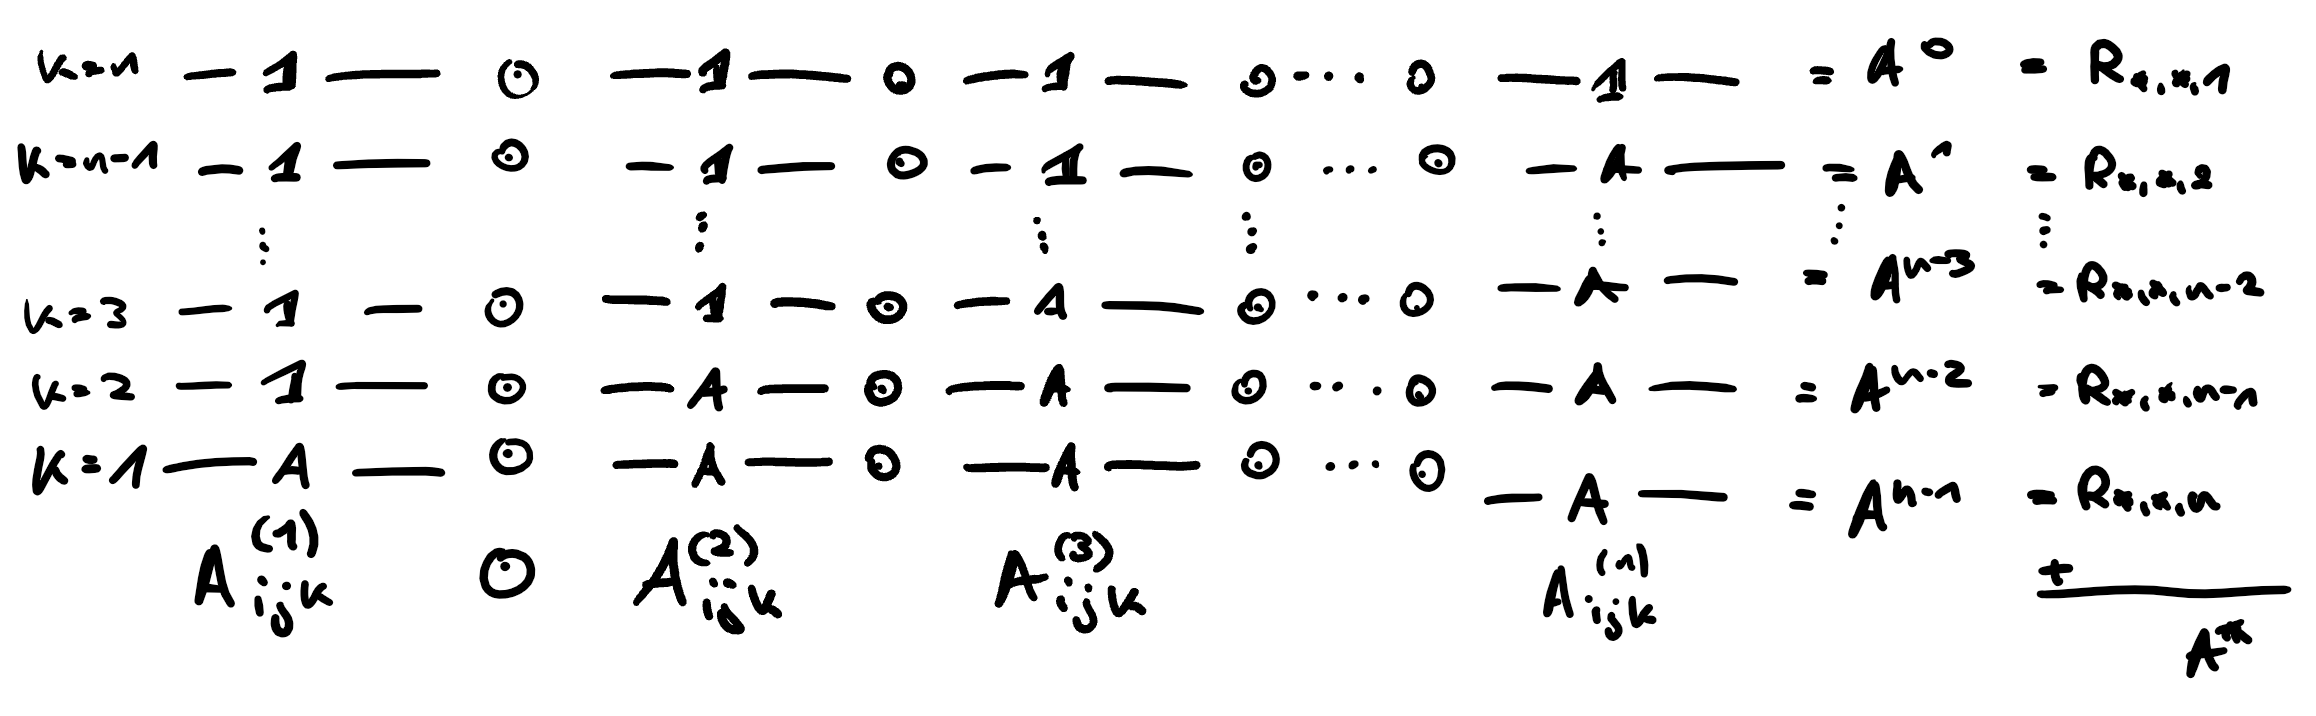
\includegraphics[width=\linewidth]{shortest_path_tensor.png}
    \caption{Visualized the shortest path tensors}
    \label{fig:shortest_path_tensor}
\end{figure}

The resulting expression comes out to be
$$A^*_{ij} = \sum_{k, t_1, \dots, t_{n-1} \in [n]} A^{(1)}_{it_1k}A^{(2)}_{t_1t_2k}A^{(3)}_{t_2t_3k}\dots A^{(n-1)}_{t_{n-2}t_{n-1}k}A^{(n)}_{t_{n-1}jk}$$
Which correspond to the Einsum string
$$it_1k, t_1t_2k, t_2t_3k, \cdots, t_{n-2}t_{n-1}k, t_{n-1}jk \to ij$$

\section{All pairs longest path}
The computation is exactly the same as in the All pairs shortest path problem. The only difference is the semiring in use. Here we need $(\R \cup \{-\infty\}, \max, +)$ and there must not exist a positive cycle. Then just compute $A^*$ and the entry $A^*_{ij}$ holds the longest path from $v_i$ to $v_j$. [Small note on convergency of $A^*$]

\section{Minimum weight spanning tree}
Here we need the observation that the edge $(v, u)$ is not included in the MST iff its weight is larger than the maximum weight of any path between $v$ and $u$. [Add proof] This we can model, by defining the weight of a path as the maximum of the weights of its edges. Then we compute the all pairs shortest path problem, but now we have exchanged the $+$-operation by the $\max$-operation, which means we have to use the $(\R \cup\{\infty\}, \min, \max)$ semiring. After computing $A^*$ we include the edge $(v_i, v_j)$ in the minimum weight spanning tree iff $A_{ij} \leq A^*_{ij}$.
[Diskuss conergency of $A^*$]

\section{Further Problems}
\begin{itemize}
    \item Marko Chaines. Using the semiring $([0, 1], +, \cdot)$ $A^k_{ij}$ holds the propability that an agent reaches $v_j$ starting at $v_i$ after $k$ steps if the weights of the edges symbolze the properbility that an agent moves along this edge.
    \item Reachability / Transitive hull. In an undirected unweighted graph, we ask the question whether a vertex $v_j$ is reachable starting at vertex $v_i$. For that we could just compute the shortest path and see whether $A^*_{ij}$ is infinite or not. But we can achieve the same with less information by just using the $(\{0, 1\}, \lor, \land)$ semiring and check whether $A^*_{ij} = 1$.
\end{itemize}
\chapter{Integer linear programs}
\section{Introduction}

\section{Preliminaries}
[Define a ILP?]

For us, it will be usefull to discuss matricies where all columns sum to the same number $\alpha$. Because we are in the framework of ILPs, we also use natural numbers as entries. So, we are interested in $A \in \N^{m \times n}$ if $\forall i \in [n]\colon \sum_{i=1}^{m}A_{ij} = \alpha$. These matricies have special properties when they are used in linear system of equations, which we will discover in the next lemma.

\begin{lemma}
    \label{lemma:ilp_pre1}
    Let $A\in \N^{m \times n}, A \neq \zeromat$ such that each column of $A$ sums up to the same number $\alpha \in \N$. Let $b \in \N^m$ arbitrary and consider the linear system of equation $Ax=b$, where $x \in \N^n$. Then, the following two statements are true

    \begin{enumerate}
        \item[(1)] For all solutions $x \in \R^n$ must hold that its components must always sum up to the same number $k$.
        \item[(2)] There only exist a solution of the components of $b$ sum up to a multiple of $\alpha$. This multiple turnes out to be $k \cdot \alpha$.
    \end{enumerate}
\end{lemma}

\begin{proof}
    $A \neq \zeromat \Rightarrow \alpha > 0$. Lets assume there exists a solution $x \in \R^n$ of the linear system of equation $Ax=b$.
    $$\sum_{i=1}^m b_i = \sum_{i=1}^{m}\sum_{j=1}^{n}A_{ij} x_j = \sum_{j=1}^{n}\underbrace{\sum_{i=1}^{m}A_{ij}}_\alpha x_j = \alpha \cdot \sum_{j=1}^{n}x_j$$
    Because $\alpha$ and $b_i$ are fixed and will not change dependent of $x$ and $\alpha \neq 0$, statement (1) immidiatly follows. Thus we have proven, if there exist a solution $x \in \N^n$, then it must hold that $\sum_{i=1}^{m}b_i = \alpha \cdot k$ which is the contraposition of (2).
\end{proof}
Reviewing the last lemma, one might hope that we can convert any system of lineare equation $Ax = b$ in another $A'x = b'$ such that in $A'$ all columns sum up to the same number and $x$ is a solution to the first if and only if it is a solution to the second. It is easy to see, that this is sadly not possible in general. For this, remember that in all solutions of $A'x=b'$, the components add up to a fixed number which must than also hold for $Ax=b$. But this property does not hold for general linear systems of equations. For example
$$
\left(\begin{matrix}
    1 & 2\\
    1 & 2
\end{matrix}\right)
x = \left(\begin{matrix}
    2\\2
\end{matrix}\right)
$$
yields among others the solutions $(2, 0)^\top$ and $(0, 1)^\top$, which clearly don't add up to the same number. 

We have to accept, that when creating the adapted system of equations, we also have to adapt the solutions. The hop is, that from the adapted solution we can recover the solutions we are looking for. This is indeed possible and is the basis for all further discussions.

\begin{theorem}
    \label{theorem:column_sum_construction}
    Let $A\in \N^{m \times n}$ such that $A$ has no zero-column and $b \in \N^m$. Then, there exists $A' \in \N^{(m+1) \times (n+1)}$ and $b' \in \N^{m+1}$ such that all columns of $A$ sum up to the same number $\alpha \in \N^*$ and for every $x \in \N^n$:
    $$Ax = b \Leftrightarrow \exists x_{n+1}\in \N\colon A' \smat{
        x_1\\
        \vdots\\
        x_n\\
        x_{n+1}
    } = b'$$
\end{theorem}

\begin{proof}
    First we need to get an upper bound in the solutions $x \in \N^n$ in $Ax=b$. We will do that similarly as in the proof of Lemma \ref{lemma:ilp_pre1}. Let $s_j = \sum_{i=0}^{m} A_{ij}$, the column sum of the $j$-th column in $A$. Let $s := \min\{s_1, \dots, s_j\}$. Because $A$ has no zero-colmns $s > 0$.
    $$\sum_{i=1}^m b_i = \sum_{i=1}^{m}\sum_{j=1}^{n}A_{ij} x_j = \sum_{j=1}^{n}\underbrace{\sum_{i=1}^{m}A_{ij}}_{s_j} x_j \geq s \cdot \sum_{j=1}^{n}x_j \Leftrightarrow \sum_{j=1}^{n}x_j \leq \frac{1}{s}\sum_{i=1}^{m}b_i$$
    Now we can construct $A'$ and $b'$. Let $\alpha \geq \max\{s_1, \dots, s_n\}$ and $v_j := \alpha - s_j$. 
    $$A' :=
    \begin{pNiceArray}{cccc}[margin] 
    \Block[draw]{3-3}{A} & & & 0 \\
    & & & \vdots\\
    & & & 0\\
    v_1 & \dots  & v_n & \alpha 
    \end{pNiceArray} \in \N^{(m+1) \times (n+1)}
    \qquad b' := \mat{b_1\\\vdots\\b_m\\\beta} \in \N^{m+1}$$
    It is clear that in $A'$, all columns sum up to $\alpha$. Observe also that $s \leq \alpha$. Because of Lemma \ref{lemma:ilp_pre1} (2) we need to set $\beta := k \cdot \alpha - \sum_{i=0}^{m}b_i$ for some $k \in \N$. We will set $k \geq \frac{1}{s}\sum_{i=1}^{m}b_i$. Thus we get $\beta \geq \frac{\alpha}{s}\sum_{i=1}^{m}b_i - \sum_{i=1}^{m}b_i \geq 0$, because $\frac{\alpha}{s} \geq 1$, which is needed, as $\beta \in \N$. Now we have to prove the equivalince:
    \begin{itemize}
        \item[``$\Leftarrow$''] Because the first $m$ rows in $A'x=b'$ are equialent to $Ax=b$ discarding the last component of the solution $x_{n+1}$ we see that the vector $(x_1, \dots, x_n)^\top$ is indeed a solution to $Ax=b$.
        \item[``$\Rightarrow$''] Let $(x_1, \dots, x_n)$ be the solution of $Ax=b$. We we have to find a $x_{n+1} \in \N$ such that $x' := (x_1, \dots x_{n+1})$ is a solution to $A'x' = b'$. 
        
        Now we'll call $(x_1, \dots, x_{n+1}) =: x'$. Because of Lemma \ref{lemma:ilp_pre1} (1) we need to set $x_{n+1} := k - \sum_{j=1}^{n}x_j$. Similarly to the discussion on $\beta$, we also have to make sure for $x_{n+1}$, that it is $\geq 0$. $x_{n+1} \geq k - \frac{1}{s}\sum_{i=1}^{m}b_i \geq \frac{1}{s}\sum_{i=1}^{m}b_i - \frac{1}{s}\sum_{i=1}^{m}b_i = 0$.
        
        Now, we need to check whether $A'x'\stackrel{?}{=}b'$. Because the first $m$ rows in $A'x'=b'$ are equialent to $Ax=b$ discarding the last component of the solution $x_{n+1}$ we only have to check the last row. So we have to prove $(A'x')_{n+1} = \beta$
        \begin{align*}
            (A'x')_{n+1} &= \sum_{j=1}^{n}v_jx_j + \alpha \cdot x_{n+1} = \sum_{j=1}^{n}(\alpha - s_j)x_j + \alpha \cdot x_{n+1} = \alpha \cdot \sum_{j=1}^{n}x_j - \sum_{j=1}^{n}s_jx_j + \alpha \cdot x_{n+1}\\
            &= \alpha \cdot \underbrace{\left(\sum_{j=1}^{n}x_j + x_{n+1}\right)}_k - \sum_{j=1}^{n}s_jx_j = \alpha \cdot k - \sum_{j=1}^{n}\sum_{i=1}^{m}A_{ij}x_j = \alpha\cdot k - \sum_{i=1}^{m}\underbrace{\sum_{j=1}^{n}A_{ij}x_j}_{b_i}\\
            &= \alpha\cdot k - \sum_{i=1}^{m}b_i = \beta
        \end{align*}
    \end{itemize}
\end{proof}
So from this point on we can w.l.o.g. assume, that in any system of equations $Ax=b$ all columns sum up to the same number.

\section{Tropic polynomials}
Let $c_{e_1, \dots, e_m}(p)$ be the coefficiant in $p \in S[q_1, \dots q_m]$ of the monomial $p_1^{e_1}\dots p_m^{e_m}$. 

\begin{lemma}
    \label{lemma:prem_trop_poly}
    Let $A \in \N^{m \times n}$ and $w \in \R^n$. Let
    $$f := \bigoplus_{i=1}^{n} \sprod{w}{\hat e_i}\odot  q_1^{(A\hat e_i)_1}\dots q_m^{(A\hat e_i)_m} \in \T[q_1, \dots, q_m]$$
    be a tropic polynomial. Then it will hold that for all $l \in \N$
    $$c_{e_1, \dots, e_m}(f^{\odot l}) = \min\left\{\sprod{w}{v} \mid v \in \N^n, \sum_{i=0}^{n}v_i = l, Av=\smat{e_1\\\vdots\\e_m}\right\}$$
    Where $\min\emptyset:=\infty$.
\end{lemma}

\begin{proof}
    We will prove it by induction over $l$.
    \begin{itemize}
        \item[$l=0$:] $f^{\odot0} = 0$. There exists only one vector in $v \in \N^n$ such that $\sum_{i=0}^{n}v_i = 0$, which is the zero vector $\vec 0$. It is also clear that $\sprod{w}{\vec 0}= 0$ and $A\vec0=0$. So
        $$
            \min\left\{\sprod{w}{v} \mid v \in \N^n, \sum_{i=0}^{n}v_i = 0, Av=\smat{e_1\\\vdots\\e_m}\right\} = \begin{cases}
                0 &\textrm{if}\quad e_1, \dots, e_m = 0\\
                \infty &\textrm{else}
            \end{cases}
            \stackrel{\checkmark}{=}c_{e_1, \dots, e_m}(0)
        $$
        \item[$l=1$:] Because $\hat e_1, \dots, \hat e_n$ are all the vectors in $\N^n$, such that their components add up to 1, the equality is true by construction.
        \item[$l>1$:] Let $e := (e_1, \dots, e_m)^\top \in \N^m$
        \begin{align*}
            c_{e_1, \dots, e_m}(f^{\odot l}) &= c_{e_1, \dots, e_m}(f^{\odot (l-1)}\odot f) = \bigoplus_{\substack{f, g \in \N^m\\f+g=e}} c_{f_1, \dots, f_m}(f^{\odot (l-1)}) \odot c_{g_1, \dots, g_m}(f)\\
            &= \bigoplus_{\substack{f, g \in \N^m\\f+g=e}} \left(\bigoplus_{\substack{x \in \N^n\\\sum_{i=1}^{n}x_i = l-1\\Ax=f}}\sprod{w}{x}\right) \odot \left(\bigoplus_{\substack{y \in \N^n\\\sum_{i=1}^{n}y_i = 1\\Ay=g}}\sprod{w}{y}\right)\\
            &= \bigoplus_{\substack{f, g \in \N^m\\f+g=e}}\bigoplus_{\substack{x, y \in \N^n\\\sum_{i=1}^{n}x_i = l-1\\\sum_{i=1}^{n}y_i = 1\\Ax=f, Ay=g}} \underbrace{\sprod{w}{x} \odot \sprod{x}{y}}_{\sprod{w}{x+y} =: \sprod{x}{v}} = \bigoplus_{\substack{f, g \in \N^m\\f+g=e}}\bigoplus_{\substack{v \in \N^n\\\sum_{i=1}^{n}v = l\\Av=f+g=e}} \sprod{w}{v}\\
            &= \bigoplus_{\substack{v \in \N^n\\\sum_{i=1}^{n}v = l\\Av=e}} \sprod{w}{v} = \min\left\{\sprod{w}{v} \mid v \in \N^n, \sum_{i=0}^{n}v_i = l, Av=e\right\}
        \end{align*} 
    \end{itemize}
\end{proof}

\begin{theorem}
    Let $\min \stackrel{!}{=} w^\top x$ s.t. $Ax=b$ an ILP, such that all columns of $A$ sum up to the same number $\alpha \in \N^*$. We wat the ILP, to have solutions, so $k = \frac{1}{\alpha}\sum_{i=1}^{m}b_i \in \N$ exists. Let $f \in \T[q_1, \dots, q_m]$ be like in Lemma \ref{lemma:prem_trop_poly}, so 
    $$f := \bigoplus_{i=1}^{n} \sprod{w}{\hat e_i}\odot  q_1^{(A\hat e_i)_1}\dots q_m^{(A\hat e_i)_m}$$
    Then $c_{b_1, \dots, b_m}(f^{\odot k})$ solves the ILP 
\end{theorem}

\begin{proof}
    Because of Lemma \ref{lemma:ilp_pre1}, for all solutions $x \in \N^n$ of $Ax=b$ will hold that $\sum_{i=1}^{n}x_i = k$. No it is just a matter of rewriting the solution of the ILP and applying Lemma \ref{lemma:prem_trop_poly}.
    \begin{align*}
        \min\{\sprod{w}{x} \mid x \in \N^n, Ax=b\} &\stackrel{\ref{lemma:ilp_pre1}}{=} \min\left\{\sprod{w}{x} \mid x \in \N^n, \sum_{i=1}^{n}x_i = k , Ax=b\right\}\\
        &\stackrel{\ref{lemma:prem_trop_poly}}{=} c_{b_1, \dots, b_m}(f^{\odot k})
    \end{align*}
\end{proof}

\section{Solving ILPs by Shortest Path}
We want to be able to solve an ILP by using the shortest path framework, so the first task is to construct a directect weighted graph $G = (V, E)$ based on an ILP ($\sprod{w}{x} \stackrel{!}{=} \min$ s.t. $Ax=b$). Again we only look at matricies, in which all columns sum up to the same number $\alpha \in \N^*$. Let $k := \frac{1}{\alpha} \sum_{i=1}^{n}x_i \in \N$. Because of Lemma \ref{lemma:ilp_pre1}, $k$ exists. Now we are ready to set the vertecies:
$$V := \left\{Ax \mid x \in \N^n, \sum_{i=1}^{n} x_i \leq k \right\}$$ 
If $Ax=b$ has solutions, we immidiatly see that $b \in V$, because the components of all solutions add up to exactly $k$. We also note that $\vec 0 = A\vec 0 \in V$. Now we can define the edges:
$$E := \{(v, u) \mid v, u \in V, u = v + A\hat e_i, i \in [n]\}$$
In other words, an edge exists, if underlying vectors only differ by an unit vector.

The resulting graph will be a tree with $\vec 0$ as the root. We will define the weight as follow:
$$w(v, v + A\hat e_i) := \sprod{w}{\hat e_i}$$
The nodes with distance $l$ will be the the nodes $Ax$ where $\sum_{i=1}^{n}x_i = l$. So the tree will have depth $k+1$. So the shortest path between $\vec 0$ and $b$ will be 

$$\min\left\{\sum_{l=1}^{k} \sprod{w}{\hat e^{(l)}} \mid \sum_{l=1}^{k}\hat Ae^{(l)} = b, \hat e^{(l)} \in \{\hat e_{1}, \dots, \hat e_n\}\right\}$$

By using the liniarity of the scalar product and the matrix multiplication and than setting $x := \sum_{l=1}^{k}\hat e^{(l)}$ this is equal to 
$$\min\left\{\sprod{w}{x} \mid x \in \N^n, \sum_{i=1}^{n}x_i = k , Ax=b\right\} \stackrel{\ref{lemma:ilp_pre1}}{=} \min\{\sprod{w}{x} \mid x \in \N^n, Ax=b\}$$
which solves th ILP.\qed

\section{Optimizing the graph algorithm}
In the last chapter, we saw that the runtine of solving ILPS in terms of a shortest path problem is heavily influenced by the number of layers in the corresponding graph. We called this number $k$ and it is equal to the sum of the components of the solutions of $Ax=b$. We needed for $A$'s columns to all sum up to the same number. If $A$ did not have this property, we could construct a new matrix $A'$ that would have this property and alters the solution space minimally. For this, we used Theorem \ref{theorem:column_sum_construction} where we were able to chose some $k$ which again drastically influences the runtime of the algorthm. There we had to put a restruction on $k$, namely
$$k \geq \frac{1}{\min_{j \in [n]} \left\{ \sum_{i=1}^{m}A_{ij}\right\}}\cdot \sum_{i=1}^{m}b_i$$
You may observe that equivalant linear systems of equations might produce different bounds. Let's look at the following simple example. We want to solve 
$$\mat{1&2\\0&6}\vec x = \mat{7\\18} \qquad \Rightarrow k \geq \frac{7 + 18}{\min\{1+0, 2+6\}} = 25$$
Meaning if we would solve an ILP with this system of linear equations we would need a graph with 25 layers. Now let's modify this system by multiplying the first row by 100:
$$\mat{100&200\\0&6}\vec x = \mat{700\\18} \qquad \Rightarrow k \geq \frac{700 + 18}{\min\{100+0, 200+6\}} = \frac{718}{100} \Rightarrow k \geq 8$$
We have achieved a major reduction of the number of layers and thus dramatically shrank the graph. In the following arguments we explore these kinds of manipulations and discover a strategy on how you would systimatically minimizing $k$. But first, we have to undestand the behavior better.

Lets first define a few helpful functions. Let $k\colon \N^{m \times n} \times \N^m \to \R$ be
$$k(A, \vec b) := \frac{1}{\min_{j \in [n]} \left\{ \sum_{i=1}^{m}A_{ij}\right\}}\cdot \sum_{i=1}^{m}b_i$$
So we need to find a $k \geq k(A, \vec b)$. Now we will generalize this function, which will be helpful later on. Let 
$$k(A, \vec b; \vec \mu) := \frac{\sprod{\vec{\mu}}{\vec b}}{\min_{j \in [m]} \sprod{\vec \mu}{\vec a_j}}$$
where $\vec a_j$ is the $j$-th column of $A$. We will restrict $\vec \mu$ as follows:
$$\vec \mu \in U_A := \{\vec x \in \R^m \mid \forall j \in [m]\colon \sprod{\vec x}{\vec a_j} > 0\}$$
Note that because all entries of $A$ are non-negative, $U_A$ is a superset of $\R_{>0}^m$. We also see that $k(A, \vec b) = k(A, \vec b; \opvec(1))$, where $\opvec(1) = (1, \dots, 1)^\top$. And also $\opvec(1) \in U_A$, because $\opvec(1) \in \R^m_{>0}$. It is left to show, why exactly this generalization is so useful. This will be handled by the next lemma
\begin{lemma}
    Let $A \in \N^{m \times n}, \vec b \in \N^m$ such that $A$ has no zero columns. Then the following to statements will hold:
    \begin{enumerate}
        \item[1)] $\forall \vec \mu \in U_A \cap \Q^m$ exist $A' \in \N^{m \times n}, \vec b' \in \N^m$, such that $\solspace(A, \vec b) = \solspace(A', \vec b')$ and
        $k(A', \vec b') = k(A, \vec b; \vec\mu)$
        \item[2)] $\forall  A' \in \N^{m \times n}, \vec b' \in \N^m$, such that $\solspace(A, \vec b) = \solspace(A', \vec b')$ exists a $\vec \mu \in U_A \cap \Q^m$, such that 
        $k(A', \vec b') = k(A, \vec b; \vec\mu)$.
    \end{enumerate}
\end{lemma}
\begin{proof}
    \begin{enumerate}
        \item[1)] Because $k(A, \vec b; \vec \mu) = k(A, \vec b; \lambda \vec \mu)$ for $\lambda > 0$ we can w.l.o.g. assuma that $\vec \mu \in \Z^m$. Because we need to construct $A'$ and $\vec b'$ such that $\solspace(A, \vec b) = \solspace(A', \vec b')$ there must exist a $C \in \GL_m(\Q)$ such that $A' = C\cdot A$ and $\vec b = C\cdot \vec b$. Thus it suffices to construct $C$. Let's chose $C$ such that
        $$C^\top \cdot \opvec(1) = \vec\mu$$
        Then it will hold that:
        \begin{align*}
            k(A', \vec b') &= k(A', \vec b'; \opvec(1)) = k(C \cdot A, C \cdot \vec b; \opvec(1))\\
            &= \frac{\sprod{\opvec(1)}{C \cdot \vec b}}{\min_{j \in [m]} \sprod{\opvec(1)}{C \cdot \vec a_j}} = \frac{\sprod{C^\top \cdot \opvec(1)}{\vec b}}{\min_{j \in [m]} \sprod{C^\top \cdot \vec \mu}{\vec a_j}}\\
            &= \frac{\sprod{\vec{\mu}}{\vec b}}{\min_{j \in [m]} \sprod{\vec \mu}{\vec a_j}} \stackrel{\checkmark}{=} k(A, \vec b; \vec\mu)
        \end{align*}
        [Reicht nicht!!!! Noch zu tun]
        It is left to show that $C \cdot A \in \N^{m \times n}$. One idea whould be the following. We know that $\vec\mu\in U_A$ thus $\sprod{\vec \mu}{\vec a_j} > 0$. Thus
        $$\opvec(1)^\top \cdot CA = (C^\top \cdot \opvec(1))^\top \cdot A = \vec\mu^\top \cdot A > \zeromat$$
        Now you could try to alter $C \mapsto C + \Delta$ iteratively such that $\Delta^\top \opvec(1) = 0$ (column sums are zero), thus $C^\top \cdot \opvec(1) = \vec\mu$ will continue to hold and somehow also garantee that $C$ stays invertable.
        \item[2)] Because $\solspace(A, \vec b) = \solspace(A', \vec b')$, there mus exist $C \in \GL_m(\Q)$ such that $A' = C \cdot A \in \N^{m \times n}$ and $\vec b' = C \cdot \vec b \in \N^m$. As in 1) we will chose $\vec \mu := C^\top \cdot \opvec(1)$ and by the calculation in 1) it will follow that $k(A', \vec b') = k(A, \vec b; \vec\mu)$. It is left to check whether $\vec \mu \in U_A$. Because $A$ had no zero columns, $A'$ also has none, which means that for every $j \in [m]$:
        $$0 < \sprod{\opvec(1)}{\vec a'_j} = \sprod{\opvec(1)}{C \cdot \vec a_j} = \sprod{C^\top \cdot \opvec(1)}{\vec a_j} = \sprod{\vec \mu}{\vec a_j} \qquad \Rightarrow\vec \mu \in U_A$$
    \end{enumerate}
\end{proof}

Statement 2) says that for any other equialent system of equations we find a $\vec \mu$ that represents its $k$-function. And statement 1) says that for every $\vec \mu$ we find a corresponding system of equations. This means that all equivalent systems of equation are exactly covered by the function $k(A, \vec b; \vec\mu)$ for some $\vec \mu$. This means, for finding the optimal $k$ we just need to minimize $k(A, \vec b; \vec \mu)$ over $\vec \mu$.

Before we proceed, one last note about continuity. Because $k(A, \vec b; \vec \mu)$ is continous when changing $\vec\mu$, we will find for every $\varepsilon > 0$ and $\vec\mu \in U_A$ a $\vec\mu' \in U_A \cap \Q^m$ such that $|k(A, \vec b; \vec \mu) - k(A, \vec b; \vec \mu')| < \varepsilon$. This means all further discussions can be done in $\R^m$.

Let's simplify notation. We will now consider $A \in \N^{m \times n}$ and $\vec b \in \N^m$ as given. And we will write $k(\vec \mu) := k(A, \vec b; \vec \mu)$ and also $U := U_A$. Our goal is to minimize $k(\vec \mu)$ over $U$.

By 2 simple observation we can allready make a lot of progress. Note that $\delta U = \{\vec x \in \R^m \mid \min_{j \in [n]}\sprod{\vec x}{\vec a_j} = 0\}$ and thus $k(\vec \mu)$ blows up to infinity when $\vec \mu \to \delta U$. Thus the minimum we are seeking cannot lie on the border of $U$. Furthermore note that $k(\vec \mu) = k(\lambda \vec\mu)$ for any $\lambda > 0$. This means that $k(\vec \mu)$ will have the same value along a ray starting at the origin. Thus it is suffictiant to only consider a $m-1$-dimensional surface of a sphere, which is compact. Remeber that any continous function on will attain its maximum and minimum at least once on a compect set. Thus we know, that any minima that will be reached are local minima in $U$.

Because we now know that we are only interested in local minima in $U$, we can start analyzing $k(\vec \mu)$ a little bit closer. But first, a little bit more notation:
$$k(\vec \mu) = \frac{\sprod{\vec{\mu}}{\vec b}}{\min_{j \in [m]} \sprod{\vec \mu}{\vec a_j}} = \sprod{\vec{\mu}}{\vec b}\cdot\max_{j \in [m]}\left\{\frac{1}{\sprod{\vec \mu}{\vec a_j}}\right\} = \max_{j \in [m]}\left\{\frac{\sprod{\vec{\mu}}{\vec b}}{\sprod{\vec \mu}{\vec a_j}}\right\} =: \max_{j\in[n]}\{k_j(\vec \mu)\}$$
and
$$U_j := \{\vec x \in U \mid \forall j' \in [n]\colon \sprod{\vec x}{\vec a_j} \leq \sprod{\vec x}{\vec a_{j'}}\}$$
So $k(\vec \mu)$ is the upper envelope of the function family $(k_j(\vec \mu))_{j \in [n]}$ and $k(\vec \mu) = k_j(\vec\mu) \Leftrightarrow \vec\mu \in U_j$ so $U_j$ is the area in $U$ where $k_j(\vec\mu)$ has the largest values. It is easy to see that $U, U_j$ are all convex thus $U$ consits of $n$ regions at max. Lets now discuss $k_j(\vec\mu)$.

\begin{lemma}
    $k_j(\vec\mu)$ is on $U$ constant or strictly monotone.
\end{lemma}
\begin{proof}
    We will split the discussion in two cases.\\
    \textbf{Case 1} $\vec a_j \parallel \vec b$: Thus $\exists c \in \R\colon \vec b = c \cdot \vec a_j$.
    $$k_j(\vec \mu) = \frac{\sprod{\vec \mu}{\vec b}}{\sprod{\vec \mu}{\vec a_j}} = \frac{\sprod{\vec \mu}{c \cdot \vec a_j}}{\sprod{\vec \mu}{\vec a_j}} = c \cdot \frac{\sprod{\vec \mu}{\vec a_j}}{\sprod{\vec \mu}{\vec a_j}} = c \qquad\Rightarrow k_j(\vec \mu)\textrm{ is constant}$$
    \textbf{Case 2} $\vec a_j \nparallel \vec b$: Thus $\lnot\exists c \in \R\colon \vec b = c \cdot \vec a_j$. We need to take the gradient. Lets first consider one component:
    $$\frac{\partial}{\partial \mu_i} k_j(\vec \mu) = \frac{b_i\sprod{\vec\mu}{\vec a_j} - \sprod{\vec\mu}{\vec b}(\vec a_j)_i}{\sprod{\vec\mu}{\vec a_j}^2} \qquad \Rightarrow \nabla_{\vec\mu} k_j(\vec\mu) = \frac{\vec b\sprod{\vec\mu}{\vec a_j} - \sprod{\vec\mu}{\vec b}\vec a_j}{\sprod{\vec\mu}{\vec a_j}^2}$$
    $$\vec 0 \stackrel{!}{=} \nabla_{\vec\mu} k_j(\vec\mu) \Rightarrow \vec b = \frac{\sprod{\vec \mu}{\vec b}}{\sprod{\vec \mu}{\vec a_j}}\vec a_j \Rightarrow \vec{a}_j \parallel \vec b$$
    Which yield a contradiction thus $k_j(\vec\mu)$ is strictly monotone.
\end{proof}

This means that the only places, where minima can exist are the edges of each $U_j$. Thus it will be interesting to look at them closer.

\begin{lemma}
    Along the shared border of $U_{j_1}, \dots, U_{j_r}$ is $k(\vec\mu)$ constant or strongly monotone.
\end{lemma}
\begin{proof}
    Because $\vec \mu \in U_{j_1}\cap \dots\cap U_{j_r}$ the following 2 statements will hold:
    $$\sprod{\vec{\mu}}{\vec a_{j_1}} = \dots = \sprod{\vec{\mu}}{\vec a_{j_r}} \quad\textrm{and}\quad k(\vec\mu) = \frac{\sprod{\vec \mu}{\vec b}}{\sprod{\vec \mu}{\vec a_{j_1}}}$$
    Now we will split the proof again into 2 cases, similar to the last proof.\\
    \textbf{Case 1} $\exists c_1, \dots, c_r \in \R\colon \vec b = c_1\vec a_{j_1} + \dots + c_1\vec a_{j_r}$.
    $$k(\vec\mu) = \frac{\sprod{\vec \mu}{\vec b}}{\sprod{\vec \mu}{\vec a_{j_1}}} = c_1 \cdot \underbrace{\frac{\sprod{\vec \mu}{\vec a_{j_1}}}{\sprod{\vec \mu}{\vec a_{j_1}}}}_1 + \dots + c_r \cdot \underbrace{\frac{\sprod{\vec \mu}{\vec a_{j_r}}}{\sprod{\vec \mu}{\vec a_{j_1}}}}_1 = c_1 + \dots + c_r \quad \Rightarrow k(\vec\mu)\textrm{ is constant}$$
    \textbf{Case 2} $\lnot\exists c_1, \dots, c_r \in \R\colon \vec b = c_1\vec a_{j_1} + \dots + c_1\vec a_{j_r}$. We want to minimize a function subject to some constraints. For that we will be using the method of Lagrange multiplieres. We have $r-1$ constraints of the following shape:
    $$\sprod{\vec\mu}{\vec a_{j_l}} = \sprod{\vec\mu}{\vec a_{j_{l+1}}} \Leftrightarrow \sprod{\vec\mu}{\vec a_{j_l} - \vec a_{j_{l+1}}} = 0, \quad l \in [r-1]$$
    Thus we get the Lagrangian
    \begin{align*}
        \lagrangian(\vec\mu, \lambda_1, \dots, \lambda_{r-1}) &= \frac{\sprod{\vec \mu}{\vec b}}{\sprod{\vec \mu}{\vec a_{j_1}}} - \sum_{l=1}^{r-1}\lambda_l \sprod{\vec\mu}{\vec a_{j_l} - \vec a_{j_{l+1}}}\\
        \vec0 \stackrel{!}{=}\nabla_{\vec \mu} \lagrangian(\vec\mu, \lambda_1, \dots, \lambda_{r-1}) &= \frac{\vec b\sprod{\vec\mu}{\vec a_{j_{1}}} - \sprod{\vec\mu}{\vec b}\vec a_{j_{1}}}{\sprod{\vec\mu}{\vec a_{j_{1}}}^2} - \sum_{l=1}^{r-1}\lambda_l(\vec a_{j_l} - \vec a_{j_{l+1}}) \\
        \Rightarrow\quad \vec0 &= \vec b\sprod{\vec\mu}{\vec a_{j_{1}}} - \sprod{\vec\mu}{\vec b}\vec a_{j_{1}} - \sprod{\vec\mu}{\vec a_{j_{1}}}^2\cdot\sum_{l=1}^{r-1}\lambda_l(\vec a_{j_l} - \vec a_{j_{l+1}})\\
        \Rightarrow\quad \vec b &= \frac{\sprod{\vec \mu}{\vec b}}{\sprod{\vec \mu}{\vec a_{j_{1}}}}\vec a_{j_{1}} + \sum_{l=1}^{r-1} \lambda_r \sprod{\vec\mu}{\vec a_{j_{1}}}(\vec a_{j_l} - \vec a_{j_{l+1}})
    \end{align*}
    Which is just a linear combination of $\vec a_{j_1}, \dots \vec a_{j_r}$, which we forbid in the first place. Thus this also yields a contradiction meaning that $k(\vec\mu)$ is strongly monotone.
\end{proof}

So have have the same situation for all $U_j$ and for its borders. Meaning that the only interesting places are the borders of the borders, in other words we want to find the places in $U$ where as many borders meet as possible. Thus if $U_1 \cup \dots \cup U_n$ is not empty, than this yields the best value.

Here we can do a small sanity check. If we again consider the case, where all columns of $A$ sum up to the same number $\alpha \in \N^*$, this means that $\alpha = \sprod{\opvec(1)}{\vec a_1} = \dots = \sprod{\opvec(1)}{\vec a_n}$ thus for these special matricies, all $U_j$ meet at $\vec \mu = \opvec(1)$, which again represents the original system of equations. Thus these systems cannot be improved, because they are allready at there minimum. Which is what we expected.

To figure out whether $U_1 \cup \dots \cup U_n = \emptyset$, we need to solve this system of equations:

\begin{align*}
    \sprod{\vec a_1 - \vec a_2}{\vec \mu} &= 0\\
    \sprod{\vec a_2 - \vec a_3}{\vec \mu} &= 0\\
    \vdots & \\
    \sprod{\vec a_{n-1} - \vec a_{n}}{\vec \mu} &= 0
\end{align*}
which has $n-1$ equations and $m$ unknowns. As $m$ is usually smaller than $n$ in the context of ILPs this actually is very likely to have solutions in $U$. But this is not ensured. Maybe algorithm... To be continued....

\subsection{Actually finding the minimum}
First we will consider the most commen case. Namely $m > n$. Also as said we will assume that $A$ as has full rank. Thus we get that $\rank(A) = n$. For the linear system of equations mentioned in the end of the last chapter we will define the matrix $M \in \Z^{(n-1) \times m}$ such that $M_{j,*} = \vec a_j - \vec a_{j+1}$. Thus the system of linear equations simplifies to
$$M\vec\mu = \vec0$$
First see that:

\begin{lemma}
    $\rank(A) = n \Rightarrow \rank(M) = n - 1$.
\end{lemma}

\begin{proof}
    We will proof this result using contraposition. $\rank(M) < n-1$ implies that there exists linear dependence of the rows in $M$. But remeber how the rows of $M$ are defined. Thus we get:
    $$\vec 0 = \sum_{j=0}^{n-1} \lambda_j (\vec a_j - \vec a_{j+1})$$
    But this is just a linear dependence of the columns in $A$. Because there are less columns than rows in $A$, this implies that $\rank(A) < n$. 
\end{proof}

Now we can simply do some dimensional analysis to figure out if we get solutions. The solutions of $M\vec\mu = \vec0$ will be by definition the kernel of $M$. We hope the the dimension of the kernel ea. the nullity is greater than 0. The Rank-nullity theorem for $M$ yields:
$$m = \rank{M} + \nullity(M) = n-1 + \nullity(M) \Leftrightarrow \nullity(M) = m - n + 1 > 0$$
Puh, we get indeed solution for $\vec\mu$ which are not just the zero-vector. But in order for $\mu$ to be a relevant solution it needs to have a positive dot-product with all $\vec a_j$. Remeber that by construction $\sprod{\vec\mu}{\vec a_j}$ will be the same for every $j$. We will call $\sprod{\vec\mu}{\vec a_j} := d$. If $d > 0$ we are done. If $d < 0$ remember that, because the linear system of equations in homogenous, if $\vec\mu$ is a solution, than $-\vec\mu$ is also a solution, which does actually yield a positive dot product. The last problem is $d = 0$. To see that we can actually always avoid this case, we we have to do more dimensional analysis:

We ask ourselfs, how many non-zero vectors exist, that produce 0 when taking the dot-product with the columns of $A$. So we care about the dimension of the solution space of the following system of equations:
$$A^\top\vec\mu = \vec0$$
Well, this is again the nullspace of $A^\top$. So we can again apply the Rank-nullity theorem for $A^\top$:
$$m = \underbrace{\rank(A^\top)}_{\rank(A)} + \nullity(A^\top) = n + \nullity(A^\top) \Leftrightarrow \nullity(A^\top) = m - n$$
This yields then phenomenal result that $\nullity(A^\top) < \nullity(M)$ which ensures that the solution space of $M\vec\mu = \vec0$ contains vectors that have a positive dot-product with all columns of $A$.

Was cool wäre, wär $\rank(A) = k \Rightarrow \rank(M) = k - 1$. okay lets try it
\begin{lemma}
    $\rank(A) = r \Rightarrow \rank(M) = r - 1$
\end{lemma}
\begin{proof}
    Let $[\vec b_1, \dots, \vec b_r]$ be the basis of the column space of $A$. We will construct $[\vec c_1, \dots, \vec c_{r-1}]$ which is supposed to be the basis of the row space of $M$. Let $\vec c_j = \vec b_j - \vec b_{j+1}$. In order for it to actually be a basis we are looking for, we need to check 2 things:
    \begin{itemize}
        \item $[\vec c_1, \dots, \vec c_{r-1}]$ is linearly independend.
        
        We will do it using contraposition. From $[\vec c_1, \dots, \vec c_{r-1}]$ being linearly dependend we will conclude that $[\vec b_1, \dots, \vec b_r]$ is also linearly dependend, which is impossible as we assumed it to be a basis. For that let 
        $$\vec 0 = \sum_{j=1}^{r-1} \lambda_j \vec c_j$$
        a linear dependence. Now we can rewrite that:
        $$\vec 0 = \sum_{j=1}^{r-1} \lambda_j \vec c_j = \sum_{j=1}^{r-1} \lambda_j (\vec b_j - \vec b_{j+1}) = \lambda_1 \vec b_1 + \sum_{j=2}^{r-1} (\lambda_j - \lambda_{j-1}) \vec b_j - \lambda_{r-1}\vec b_r =: \sum_{j=1}^{r} \lambda'_j \vec b_j$$
        with $\lambda'_1 = \lambda_1$, $\lambda'_r = -\lambda_{r-1}$ and $\lambda'_j = \lambda_j - \lambda_{j-1}$ for $j \in \{2, \dots, r-1\}$. Now we have to check that at least one $\lambda'_j$ is not 0. Let $l$ be the smallest index, such that $\lambda_l \neq 0$. If $l=1$ than $\lambda'_1 = \lambda_1 \neq 0$ and if $l > 1$, then $\lambda_{l-1} = 0$ and thus $\lambda'_l = \lambda_l - \lambda_{l-1} = \lambda_l \neq 0$, which yields a linear dependence for $[\vec b_1, \dots, \vec b_r]$ and thus the desired contradiction.
        \item $\Span(\vec c_1, \dots, \vec c_{r-1})$ is actually the row space. 
        
        This, we will do in 2 steps. Let the row space of $M$ be $R$ and let $C := \Span(\vec c_1, \dots, \vec c_{r-1})$.
        \begin{enumerate}
            \item[$C \subseteq R$:]
        \end{enumerate}
    \end{itemize}
\end{proof}

\subsection{Actually finding the minimum (2nd try)}
We will give the linear system of equations of the last chapter a name. Because in this chapter, it is all about the question, whether a suitable solution exists. First let $\vec b_j = \vec a_j - \vec a_{j+1}$ for $j \in [n-1]$ and let $M \in \Z^{(n-1) \times m}$ such that the $j$-th row of $M$ is $\vec b_j$. This way we can rewrite the abovementioned system of equations:
$$M\vec\mu = \vec0$$
The matrix $M$ has a nice property, which we will abuse in this section:
\begin{lemma}
    Let $r:= \rank(A)$. Then $r-1 \leq \rank(M) \leq r$.
\end{lemma}
\begin{proof}
    Here we will not determine $\rank(M)$ but $\rank(M^\top)$ which is well known to be the same. Furthermore we will use that the rank of the matrix is the dimensionof its column space. Plugging in the definitions of $A$ and $M$, we can reframe the lemma:
    \begin{align*}
        r &= \dim(\Span(\vec a_1, \dots, \vec a_n))\\
        s &:= \dim(\Span(\vec b_1, \dots, \vec b_{n-1})) = \dim(\Span(\vec a_1 - \vec a_2, \dots, \vec a_{n-1} - \vec a_n))
    \end{align*}
    $$\textrm{To show: } r-1 \leq s \leq r$$
    \begin{enumerate}
        \item[$s\leq r$:] Because all $\vec b_j$ are linear combinations of $\vec a_j$'s, we immediatly get that
        $$\Span(\vec b_1, \dots, \vec b_{n-1}) \subseteq \Span(\vec a_1, \dots, \vec a_n)$$
        which immediatly results in $s\leq r$.
        \item[$r-1 \leq s$:] We know that we can find $r$ linearly independend $\vec a_j$'s. Let the set of these vectors be $S := \{\vec a_{j_1}, \dots, \vec a_{j_r}\}$. If $\vec a_n$ is in $S$ we need to drop this element, ia $S := S \setminus \{\vec a_n\}$. Thus we get that $|S| \geq r-1$. Now the goal is to find $r-1$ linearly independend $\vec b_j$'s. We will chose $\vec b_{j_1}, \dots, \vec b_{j_{r-1}}$. It is left to show, that they are indeed linearly independend.
        
        For that, we will assume that they are actually dependend and conclude that $\vec a_{j_1}, \dots, \vec a_{j_{r-1}}$ are also dependend which we assumed otherwise. That beeing said, as $\vec b_{j_1}, \dots, \vec b_{j_{r-1}}$ are assumed to be linearly dependend, there exist $\lambda_1, \dots, \lambda_{r-1}$ such that:
        \begin{align*}
            \vec0 &= \sum_{l=1}^{r-1}\lambda_{l}\vec b_{j_l}\\
            &= \sum_{l=1}^{r-1}\lambda_{l}(\vec a_{j_l} - \vec a_{j_l+1})
        \end{align*}


    \end{enumerate}
\end{proof}

\subsection{3rd try - Explore the solution space}
We will give the linear system of equations of the last chapter a name. Because in this chapter, it is all about the question, whether a suitable solution exists. First let $\vec b_j = \vec a_j - \vec a_{j+1}$ for $j \in [n-1]$ and let $M \in \Z^{(n-1) \times m}$ such that the $j$-th row of $M$ is $\vec b_j$. This way we can rewrite the abovementioned system of equations:
$$M\vec\mu = \vec0$$
Through dimensional analysis we can figure out when it is ensured that suitable solution exist. The dimension of the solution space is the nullity of $M$. To determine this, we can use the Rank-nullity theorem:
$$m = \rank{M} + \nullity(M) \Leftrightarrow \nullity(M) = m - \rank{M}$$
But in order for $\mu$ to be a relevant solution it needs to have a positive dot-product with all $\vec a_j$. Remeber that by construction $\sprod{\vec\mu}{\vec a_j}$ will be the same for every $j$. We will call $\sprod{\vec\mu}{\vec a_j} := d$. If $d > 0$ we are done. If $d < 0$ remember that, because the linear system of equations in homogenous, if $\vec\mu$ is a solution, than $-\vec\mu$ is also a solution, which does actually yield a positive dot product. The last problem is $d = 0$. To see that we can actually always avoid this case, we we have to do more dimensional analysis:

We ask ourselfs, how many non-zero vectors exist, that produce 0 when taking the dot-product with the columns of $A$. So we care about the dimension of the solution space of the following system of equations:
$$A^\top\vec\mu = \vec0$$
Well, this is again the nullspace of $A^\top$. So we can again apply the Rank-nullity theorem for $A^\top$. Remeber from here on that we can use $\rank(A) = \rank(A^\top)$ so I will exchange these a matrix for its transpose regularly.
$$m = \rank{A^\top} + \nullity(A^\top) \Leftrightarrow \nullity(A^\top) = m - \rank{A}$$
If the nullity of $A\top$ is less then the nullity of $M$ we will always get a suitable solution for $\mu$ because there would be just not enough unsuitable solutions. This inequality can be restated as follows:
$$\nullity(M) > \nullity(A^\top) \Leftrightarrow m - \rank(M) > m - \rank(A) \Leftrightarrow \rank(M) < \rank(A)$$
The hope is, that this is always the case, so we can ensure the existance of solutions. But we will see that it is not that easy.

Let's collect some facts about the two matricies:
\begin{lemma}
    $\rank(M) \leq \rank(A)$
\end{lemma}
\begin{proof}
    We will use that the rank of the matrix is the dimensionof its column space. Because all $\vec b_j$ are linear combinations of $\vec a_j$'s, we immediatly get that
    $$\Span(\vec b_1, \dots, \vec b_{n-1}) \subseteq \Span(\vec a_1, \dots, \vec a_n)$$
    which immediatly results in $\rank(M^\top) \leq \rank(A)$.
\end{proof}

\begin{lemma}
    If all $\vec a_j$ are linearly independend, then $\rank(M) < \rank(A)$.
\end{lemma}
\begin{proof}
    We will prove the contraposition. Because the last lemma prohibits $\rank(M) > \rank(A)$, the contraposition states that
    $$\rank(M) = \rank(A) \Rightarrow \vec a_j \textrm{ are linearly dependend}$$
    $\rank(M) = \rank(M^\top) = \rank(A)$ implies that $\dim(\Span(\vec b_1, \dots, \vec b_{n-1})) = \dim(\Span(\vec a_1, \dots, \vec a_n))$.\\
    But as $\Span(\vec b_1, \dots, \vec b_{n-1}) \subseteq \Span(\vec a_1, \dots, \vec a_n)$, we actually get that:
    $$\Span(\vec b_1, \dots, \vec b_{n-1}) = \Span(\vec a_1, \dots, \vec a_n)$$
    So we see that the spaces that is spanned by $\vec a_j$'s can be spanned by using one vector less, so the $\vec a_j$'s have to be linearly dependend.
\end{proof}

The last lemma actually ensures, that if all $\vec a_j$'s are linearly independed, we always will get a suitable solution $\mu$ by solving the system of equations. It is left to discuss, what happens if this is not the case:

\begin{lemma}
    If $\rank(M) = \rank(A)$ than the linear system of equations $M\vec\mu = \vec0$ yields no solution such that $\sprod{\vec a_j}{\vec\mu} > 0$ for all $j$ (so no suitable solution).
\end{lemma}

\begin{proof}
    We will do this by actually showing that $\{\vec\mu\mid M\vec\mu = \vec0\} = \{\vec\mu\mid \sprod{\vec a_j}{\vec\mu} = 0\}$. We see that the LHS is just $\ker(M)$ and the RHS the $\ker(A^\top)$. Thus we need to show that:
    $$\ker(M) = \ker(A^\top)$$
    In a previous proof we already saw that $\rank(M) = \rank(A)$ results in 
    $$\Span(\vec b_1, \dots, \vec b_{n-1}) = \Span(\vec a_1, \dots, \vec a_n)$$
    Here the LHS is just $\im(M^\top)$ and the RHS is $\im(A)$. For any matrix it will hold that $\im(A) = \ker(A^\top)^\perp$. Applying this, we get $\ker(M)^\perp = \ker(A^\top)^\perp$. For an finite-dimensioal vector space $V$, it holds that $(V^\perp)^\perp = V$, which when applied yields $\ker(M) = \ker(A^\top)$. The result we were looking for.
\end{proof}

\subsection{Developing the algorithm}
In the last chapter we saw, if all $\vec a_j$ are linearly independend, we actually suitable $\vec\mu$, the problem obviously beeing that we cannot assume that all $\vec a_j$ are linearly independend. For example, it is very common for the matrix $A$ to be wider than high, which imidiatly produces linearly dependend $\vec a_j$'s. So now we need a way to handle general matrices, in particular those where the $\vec a_j$'s are linearly dependend. 

We will start of with a solution not necessary the best one. Then, we will show that it cannot be improved. Let's choose a basis out of $\vec a_j$. Let this basis be $[\vec a_{j_1}, \dots, \vec a_{j_r}]$. Then we will construct a matrix $A' \in \N^{m \times r}$ that only contains those basis vectors as columns. If we build its difference matrix $M'$ we know that:
\begin{enumerate}
    \item $\rank(M') < \rank(A')$
    \item We will get a $\vec\mu$ such that $\sprod{\vec a_{j_1}}{\vec\mu} = \dots = \sprod{\vec a_{j_r}}{\vec\mu} =: d > 0$ (thus a suitable solution)
\end{enumerate}
The question is still, whether the dot product is positive even with all other $\vec a_j$'s, that are not included in the basis. Let $\vec a_l$ be such a vector. Because $[\vec a_{j_1}, \dots, \vec a_{j_r}]$ is a basis, $\vec a_l$ is representable as a linear combination of these basis vectors. Now lets consider the dot product:
$$\sprod{\vec a_l}{\vec\mu} = \largesprod{\sum_{k=1}^{r}\lambda_k \vec a_{j_k}}{\vec\mu} = \sum_{k=1}^{r}\lambda_k \underbrace{\sprod{\vec a_{j_k}}{\vec\mu}}_d = d\cdot \sum_{k=1}^{r}\lambda_k$$
Thus the sign of the dot-product only depends on the coefficiants in the linear combination of the vector. And we can actaully ensure that the sum of the coefficiant is positive, by sorting the columns of $A$ by there column sum in an ascending order. 
\begin{lemma}
    Let $A$ be a matrix, where all column sums are positive and the columns are sorted in an ascending order by their column sum. Let $[\vec a_{j_1}, \dots, \vec a_{j_r}]$ be a basis of the columns space, calculated using the method of basis selection. Let $\vec a_l$ be any column of $A$, that did not get selected by the basis selection. Let $\vec\mu \in \R^m$ be a vector such that $\sprod{\vec a_{j_1}}{\vec\mu} = \dots = \sprod{\vec a_{j_r}}{\vec\mu} =: d > 0$. Then it will hold, that 
    $$\sprod{\vec a_l}{\vec\mu} \geq d$$
\end{lemma}
\begin{proof}
    As $\vec a_l$ was not selected as a basis, we know that it linearly dependend on the columns on its left in the matrix $A$. Let the set of basis vectors that are on the left of $\vec a_l$ be $\{\vec a_{j_1}, \dots, \vec a_{j_s}\}$. Because it is linearly dependend on those previous columns and the vectors $\vec a_{j_1}, \dots, \vec a_{j_s}$ are a basis of that space, we know that there must exist $\lambda_1, \dots, \lambda_s$ such that:
    $$\sum_{k=1}^{s}\lambda_k \vec a_{j_k} = \vec a_l$$
    Now we will consider the component sum of $\vec a_l$
    \begin{align*}
        \sum_{i=1}^{m} (\vec a_l)_i &= \sum_{i=1}^{m} \left(\sum_{k=1}^{s}\lambda_k \vec a_{j_k}\right)_i = \sum_{i=1}^{m} \sum_{k=1}^{s}\lambda_k \left(\vec a_{j_k}\right)_i = \sum_{k=1}^{s} \lambda_k \cdot\underbrace{\sum_{i=1}^{m} \left(\vec a_{j_k}\right)_i}_{\leq \sum_{i=1}^{m} (\vec a_l)_i}\\
        &\leq \sum_{k=1}^{s} \lambda_k \cdot\sum_{i=1}^{m} (\vec a_l)_i = \left(\sum_{k=1}^{s} \lambda_k\right) \cdot\left(\sum_{i=1}^{m} (\vec a_l)_i\right)\\
        \Rightarrow\quad 1 &\leq \sum_{k=1}^{s} \lambda_k
    \end{align*}
    With this result we are ready to compute the dot product.
    $$\sprod{\vec a_l}{\vec\mu} = \largesprod{\sum_{k=1}^{s}\lambda_k \vec a_{j_k}}{\vec\mu} = \sum_{k=1}^{s}\lambda_k \underbrace{\sprod{\vec a_{j_k}}{\vec\mu}}_d = d\cdot \underbrace{\sum_{k=1}^{s}\lambda_k}_{\geq 1} \geq d$$
\end{proof}

Now we know if we only make sure that the columns of $A$ are ordered by their column sum, that any solution we get by first applying basis selection will ensure a positive dot-product with any $\vec a_j$, not only the basis vectors. But the previous result is even stronger than that. It says that any other dot-product is actaully at least as big as the dot-product with the basis vectors. Why is this important? Remember that we wanted to minize the function:
$$k(\vec \mu) = \frac{\sprod{\vec{\mu}}{\vec b}}{\min_{j \in [m]}\sprod{\vec\mu}{\vec a_j}}$$
If we plug in the $\vec\mu$ we found using the algorithm, we know that $d$ is this the smallest dot-product, which yields the result, that for any $\vec\mu$ resulting from this algorithm, it will hold that
$$k(\vec \mu) = \frac{1}{d}\cdot\sprod{\vec{\mu}}{\vec b}$$
The found $\vec\mu$ is in $U_{j_1} \cap \dots \cap U_{j_r}$. But because $[\vec a_{j_1}, \dots, \vec a_{j_r}]$ und thus $\vec b$ is a linear combination of those, $k(\vec\mu)$ is constant there. So adding other vectors aprt from these basis vectors wont help.

The last question is, whether if we select a different basis, if then $k(\vec\mu)$ can achieve a lower value. This will be handled by the next lemma.

\begin{lemma}
    Let $A$ be a matrix, where all column sums are positive and the columns are sorted in an ascending order by their column sum. Let $[\vec a_{j_1}, \dots, \vec a_{j_r}]$ be a basis of the columns space, calculated using the method of basis selection. Let $[\vec a_{j'_1}, \dots, \vec a_{j'_r}]$ be a different basis. Let $\vec\mu, \vec\mu' \in \R^m$ be vectors such that $\sprod{\vec a_{j_1}}{\vec\mu} = \dots = \sprod{\vec a_{j_r}}{\vec\mu} =: d > 0$ and $\sprod{\vec a'_{j_1}}{\vec\mu'} = \dots = \sprod{\vec a_{j'_r}}{\vec\mu'} =: d' > 0$. We will also assume that $k(\vec \mu) = \frac{1}{d}\cdot\sprod{\vec{\mu}}{\vec b}$ and $k(\vec \mu') = \frac{1}{d'}\cdot\sprod{\vec{\mu}'}{\vec b}$. Then $k(\vec\mu) = k(\vec\mu')$.
\end{lemma}
\begin{proof}
    Let $\vec a_{j'_r}$ be the vector in the second basis with the highest column sum. Because the first basis selected the smallest column sums, the column sum of $\vec a_{j'_r}$ is larger than any of the first basis vectors. For $k(\vec \mu') = \frac{1}{d'}\cdot\sprod{\vec{\mu}}{\vec b}$ it must hold that
    $$\forall i \in [r]\colon \sprod{\vec a_{j_i}}{\vec\mu'} \geq \sprod{\vec a_{j'_r}}{\vec\mu'} = d'$$
    but because $[\vec a_{j_1}, \dots, \vec a_{j_r}]$ is a basis, there exists a linear combination for $\vec a_{j'_r}$:
    $$\vec a_{j'_r} = \sum_{k=1}^{r}\lambda_k\vec a_{j_k}$$
    Now lets consider $d'$:
    $$d' = \sprod{\vec a_{j'_r}}{\vec\mu'} = \sum_{k=1}^{r}\lambda_k\underbrace{\sprod{\vec a_{j_k}}{\vec\mu'}}_{\geq d'} \geq d'\cdot \sum_{k=1}^{r}\lambda_k \quad\Rightarrow 1 \geq \sum_{k=1}^{r}\lambda_k$$
    On the other hand, we can consider the component sum of $\vec a_{j'_r}$:
    \begin{align*}
        \sum_{i=1}^{m} (\vec a_{j'_r})_i &= \sum_{i=1}^{m} \left(\sum_{k=1}^{r}\lambda_k \vec a_{j_k}\right)_i = \sum_{i=1}^{m} \sum_{k=1}^{r}\lambda_k \left(\vec a_{j_k}\right)_i = \sum_{k=1}^{r} \lambda_k \cdot\underbrace{\sum_{i=1}^{m} \left(\vec a_{j_k}\right)_i}_{\leq \sum_{i=1}^{m} (\vec a_{j'_r})_i}\\
        &\leq \sum_{k=1}^{r} \lambda_k \cdot\sum_{i=1}^{m} (\vec a_{j'_r})_i = \left(\sum_{k=1}^{r} \lambda_k\right) \cdot\left(\sum_{i=1}^{m} (\vec a_{j'_r})_i\right)\\
        \Rightarrow\quad 1 &\leq \sum_{k=1}^{r} \lambda_k
    \end{align*}
    These 2 results combined give us an important insight:
    $$1 = \sum_{k=1}^{r} \lambda_k$$
    Now remember that $\sprod{\vec a_{j'_r}}{\vec\mu'} = \sum_{k=1}^{r}\lambda_k\sprod{\vec a_{j_k}}{\vec\mu'}$ where we can multiply (our) 1 on the LHS and receive:
    $$\sum_{k=1}^{r}\lambda_k\sprod{\vec a_{j'_r}}{\vec\mu'} = \sum_{k=1}^{r}\lambda_k\sprod{\vec a_{j_k}}{\vec\mu'}$$
    If we compare these sums addend by addend, we will se by assumption that for all $k$ it holds that $\lambda_k\sprod{\vec a_{j'_r}}{\vec\mu'} \leq \lambda_k\sprod{\vec a_k}{\vec\mu'}$. Thus these sums can only be the same iff $\lambda_k\sprod{\vec a_{j'_r}}{\vec\mu'} = \lambda_k\sprod{\vec a_k}{\vec\mu'} \Rightarrow \sprod{\vec a_{j'_r}}{\vec\mu'} = \sprod{\vec a_k}{\vec\mu'}$ for all $k$. Thus $\vec\mu' \in U_{j_1} \cap \dots \cap U_{j_r}$, and because $k(\vec\mu)$ is constant there, we get that $k(\vec\mu) = k(\vec\mu')$.
\end{proof}

\begin{lemma}
    \textit{Improved version of prvious lemma} Let $A$ be a matrix, where all column sums are positive and the columns are sorted in an ascending order by their column sum. Let $[\vec a_{j_1}, \dots, \vec a_{j_r}]$ be a basis of the columns space, calculated using the method of basis selection. Let $[\vec a_{j'_1}, \dots, \vec a_{j'_r}]$ be a different basis, such that it is also sorted by their column sums ascendingly. Let $\vec\mu, \vec\mu' \in \R^m$ be vectors such that $\sprod{\vec a_{j_1}}{\vec\mu} = \dots = \sprod{\vec a_{j_r}}{\vec\mu} =: d > 0$ and $\sprod{\vec a'_{j_1}}{\vec\mu'} = \dots = \sprod{\vec a_{j'_r}}{\vec\mu'} =: d' > 0$. We will also assume that $k(\vec \mu) = \frac{1}{d}\cdot\sprod{\vec{\mu}}{\vec b}$ and $k(\vec \mu') = \frac{1}{d'}\cdot\sprod{\vec{\mu}'}{\vec b}$. Then it will hold that
    $$\sum_{i=1}^{m}(\vec a_{j_k})_i = \sum_{i=1}^{m}(\vec a_{j'_k})_i$$
    Meaning that we have the same distribution of column sums in both basis.
\end{lemma}
\begin{proof}
    We will do the proofe in 3 steps:
    \begin{enumerate}
        \item Show that for any basis vector of the second basis, its coordinates in the first basis sum up to 1.
        \item Show that the sum of the column sums in both basis are equal, in other words:
        $$\sum_{k=1}^{r}\sum_{i=1}^{m}(\vec a_{j_k})_i = \sum_{k=1}^{r}\sum_{i=1}^{m}(\vec a_{j'_k})_i$$
        \item Show that this results in the result we are seeking, namely:
        $$\sum_{i=1}^{m}(\vec a_{j_k})_i = \sum_{i=1}^{m}(\vec a_{j'_k})_i$$
    \end{enumerate}
    Let's start. Let's pick any basis vector of the second basis $\vec a_{j'_l}$. Obviously there exists a unique linear combination of the vectors in the first basis:
    $$\vec a_{j'_l} = \sum_{k=1}^{r}\lambda_k\vec a_{j_k}$$
    If $\vec a_{j'_l}$ is also in the first basis, meaning that there exists a $s$ such that $\vec a_{j'_l} = \vec a_{j_s}$, that it will hold that $\lambda_s = 1$ and all other $\lambda_k$'s are zero. Thus
    $$\sum_{k=1}^{r}\lambda_k = 1$$

    Now we have to consider the case where $\vec a_{j'_l}$ is not part of the first basis. As $\vec a_{j'_l}$ has not been selected in the choice of basis algorithm, it must be a linear combination of the basis vectors in the first basis that stand left in the sorted matrix. Thus:
    $$\vec a_{j'_l} = \sum_{k=1}^{s}\lambda_k\vec a_{j_k} \qquad\textrm{with}\quad \forall k \leq s\colon\sum_{i=1}^{m}(\vec a_{j_k})_i \leq \sum_{i=1}^{m}(\vec a_{j'_l})_i$$
    This result yields us following when considering the column sum of $\vec a_{j'_l}$:
    \begin{align*}
        \sum_{i=1}^{m} (\vec a_{j'_l})_i &= \sum_{i=1}^{m} \left(\sum_{k=1}^{s}\lambda_k \vec a_{j_k}\right)_i = \sum_{i=1}^{m} \sum_{k=1}^{s}\lambda_k \left(\vec a_{j_k}\right)_i = \sum_{k=1}^{s} \lambda_k \cdot\underbrace{\sum_{i=1}^{m} \left(\vec a_{j_k}\right)_i}_{\leq \sum_{i=1}^{m} (\vec a_{j'_l})_i}\\
        &\leq \sum_{k=1}^{s} \lambda_k \cdot\sum_{i=1}^{m} (\vec a_{j'_l})_i = \left(\sum_{k=1}^{s} \lambda_k\right) \cdot\left(\sum_{i=1}^{m} (\vec a_{j'_l})_i\right)\\
        \Rightarrow\quad 1 &\leq \sum_{k=1}^{s} \lambda_k = \sum_{k=1}^{r} \lambda_k
    \end{align*}
    The last step - replacing $r$ with $s$ - just corresponds with the fact, that the linear combination of the basis vectors is unique. And as we have found one, that only include the first $s$ basis vectors, we know that $\lambda_{s+1} = \dots = \lambda_r = 0$.

    Now remind yourself that, it must hold that $k(\vec \mu') = \frac{1}{d'}\cdot\sprod{\vec{\mu}'}{\vec b}$ by assumption. This only happens, if $\sprod{\vec a_{j'_l}}{\vec\mu'} = d'$ gives the smallest dot-product. So all other dot-products are actually bigger. This we can also use:
    $$d' = \sprod{\vec a_{j'_l}}{\vec\mu'} = \sum_{k=1}^{s}\lambda_k\underbrace{\sprod{\vec a_{j_k}}{\vec\mu'}}_{\geq d'} \geq d'\cdot \sum_{k=1}^{s}\lambda_k \quad\Rightarrow 1 \geq \sum_{k=1}^{s}\lambda_k = \sum_{k=1}^{r}\lambda_k$$
    Combining these two results yields again
    $$\sum_{k=1}^{r}\lambda_k = 1$$
    which completes step 1 in the proof.

    The second steps consists only of juggeling a lot a linear combinations. Lets redefine $\lambda$ for this case. Let $\lambda_{kl}$ be such that:
    $$\vec a_{j'_k} = \sum_{l=1}^{r}\lambda_{kl}\vec a_{j_l}$$
    The last result kan be thus restated:
    $$\forall k \leq r\colon\sum_{l=1}^{r}\lambda_{kl} = 1$$
    Now we just need to plug everything in we currently know:
    \begin{align*}
        \sum_{k=1}^{r}\sum_{i=1}^{m}(\vec a_{j'_k})_i &= \sum_{k=1}^{r}\sum_{i=1}^{m}\left(\sum_{l=1}^{r}\lambda_{kl}\vec a_{j_l}\right)_i = \sum_{k=1}^{r}\sum_{i=1}^{m}\sum_{l=1}^{r}\lambda_{kl}\left(\vec a_{j_l}\right)_i
    \end{align*}
\end{proof}


\begin{lemma}
    \textit{Second try}
    Let $A$ be a matrix, where all column sums are positive and the columns are sorted in an ascending order by their column sum. Let $[\vec a_{j_1}, \dots, \vec a_{j_r}]$ be a basis of the columns space, calculated using the method of basis selection. Let $[\vec a_{j'_1}, \dots, \vec a_{j'_r}]$ be a different basis, also such that the vectors are sorted based on their column sum ascendingly. Let $\vec\mu, \vec\mu' \in \R^m$ be vectors such that $\sprod{\vec a_{j_1}}{\vec\mu} = \dots = \sprod{\vec a_{j_r}}{\vec\mu} =: d > 0$ and $\sprod{\vec a_{j'_1}}{\vec\mu'} = \dots = \sprod{\vec a_{j'_r}}{\vec\mu'} =: d' > 0$. We will also assume that $k(\vec \mu) = \frac{1}{d}\cdot\sprod{\vec{\mu}}{\vec b}$ and $k(\vec \mu') = \frac{1}{d'}\cdot\sprod{\vec{\mu}'}{\vec b}$. Then $k(\vec\mu) = k(\vec\mu')$.
\end{lemma}
\begin{proof}
    We will show that not only $\sprod{\vec a'_{j_1}}{\vec\mu'} = \dots = \sprod{\vec a_{j'_r}}{\vec\mu'} = d'$ but this also holds for the first basis, namely $\sprod{\vec a_{j'_1}}{\vec\mu'} = \dots = \sprod{\vec a_{j'_r}}{\vec\mu'} = d'$. From this, is it clear that $\vec\mu' \in U_{j_1} \cap \dots U{j_r}$ and because $\restrict{k}{U_{j_1} \cap \dots U{j_r}}$ is constant and also $\vec\mu \in U_{j_1} \cap \dots U{j_r}$, we can conclude that $k(\vec\mu) = k(\vec\mu')$. So in the following we will show that indeed $\sprod{\vec a_{j'_1}}{\vec\mu'} = \dots = \sprod{\vec a_{j'_r}}{\vec\mu'} = d'$:

    Let $\vec a_{j'_l}$ be an arbetrairy vector of the second basis. Obviously there exists a unique linear combination of the vectors in the first basis:
    $$\vec a_{j'_l} = \sum_{k=1}^{r}\lambda_k\vec a_{j_k}$$
    If $\vec a_{j'_l}$ is also in the first basis, meaning that there exists a $s$ such that $\vec a_{j'_l} = \vec a_{j_s}$, that it will hold that $\lambda_s = 1$ and all other $\lambda_k$'s are zero. Thus
    $$\sum_{k=1}^{r}\lambda_k = 1$$

    Now we have to consider the case where $\vec a_{j'_l}$ is not part of the first basis. As $\vec a_{j'_l}$ has not been selected in the choice of basis algorithm, it must be a linear combination of the basis vectors in the first basis that stand left in the sorted matrix. Thus:
    $$\vec a_{j'_l} = \sum_{k=1}^{s}\lambda_k\vec a_{j_k} \qquad\textrm{with}\quad \forall k \leq s\colon\sum_{i=1}^{m}(\vec a_{j_k})_i \leq \sum_{i=1}^{m}(\vec a_{j'_l})_i$$
    This result yields us following when considering the column sum of $\vec a_{j'_l}$:
    \begin{align*}
        \sum_{i=1}^{m} (\vec a_{j'_l})_i &= \sum_{i=1}^{m} \left(\sum_{k=1}^{s}\lambda_k \vec a_{j_k}\right)_i = \sum_{i=1}^{m} \sum_{k=1}^{s}\lambda_k \left(\vec a_{j_k}\right)_i = \sum_{k=1}^{s} \lambda_k \cdot\underbrace{\sum_{i=1}^{m} \left(\vec a_{j_k}\right)_i}_{\leq \sum_{i=1}^{m} (\vec a_{j'_l})_i}\\
        &\leq \sum_{k=1}^{s} \lambda_k \cdot\sum_{i=1}^{m} (\vec a_{j'_l})_i = \left(\sum_{k=1}^{s} \lambda_k\right) \cdot\left(\sum_{i=1}^{m} (\vec a_{j'_l})_i\right)\\
        \Rightarrow\quad 1 &\leq \sum_{k=1}^{s} \lambda_k = \sum_{k=1}^{r} \lambda_k
    \end{align*}
    The last step - replacing $r$ with $s$ - just corresponds with the fact, that the linear combination of the basis vectors is unique. And as we have found one, that only include the first $s$ basis vectors, we know that $\lambda_{s+1} = \dots = \lambda_r = 0$

    Now remind yourself that, it must hold that $k(\vec \mu') = \frac{1}{d'}\cdot\sprod{\vec{\mu}'}{\vec b}$ by assumption. This only happens, if $\sprod{\vec a_{j'_l}}{\vec\mu'} = d'$ gives the smallest dot-product. So all other dot-products are actually bigger. This we can also use:
    $$d' = \sprod{\vec a_{j'_l}}{\vec\mu'} = \sum_{k=1}^{s}\lambda_k\underbrace{\sprod{\vec a_{j_k}}{\vec\mu'}}_{\geq d'} \geq d'\cdot \sum_{k=1}^{s}\lambda_k \quad\Rightarrow 1 \geq \sum_{k=1}^{s}\lambda_k = \sum_{k=1}^{r}\lambda_k$$
    Combining these two results yields again
    $$\sum_{k=1}^{r}\lambda_k = 1$$

    The second step involves some change of basis. We have seen that the coordinates of the second basis vectors based on the first basis add up to 1. Let $T$ be the change of basis matrix from the second basis to the first. The abovementioned property can be reframed, as that the column sum of every colum in $T$ is equal to 1. Or in other words that $\opvec(1)^\top T = \opvec(1)^\top$. This property also holds for its inverse, because of this:
    $$\opvec(1)^\top T = \opvec(1)^\top \Leftrightarrow \opvec(1)^\top T\cdot T^{-1} = \opvec(1)^\top\cdot T^{-1} \Leftrightarrow \opvec(1)^\top = \opvec(1)^\top\cdot T^{-1}$$
    Thus if you express a vector from the first basis in coordinates of the second basis, the compoennt sums ends up to be 1 as well. Let $\vec a_{j_l}$ be an arbetrairy vector from the first basis. We thus know that
    $$\vec a_{j_l} = \sum_{k=1}^{r}\lambda'_k \vec a_{j'_k} \qquad \textrm{with}\quad \sum_{k=1}^{r}\lambda'_k = 1$$
    And here comes the final stretch:
    $$\sprod{\vec a_{j_l}}{\vec\mu'} = \largesprod{\sum_{k=1}^{r}\lambda'_k \vec a_{j'_k}}{\vec\mu'} = \sum_{k=1}^{r} \lambda'_k \underbrace{\sprod{\vec a_{j'_k}}{\vec\mu'}}_{=d'} = d' \cdot \underbrace{\sum_{k=1}^{r} \lambda'_k}_{=1} = d'$$
\end{proof}

So the algorithm is very simple
\begin{enumerate}
    \item Sort all columns in $A$ by their column sum - $O(n \log n + m \cdot n)$
    \item Do choice of basis (wich is basically gauß) - $O(m^2 \cdot n)$
    \item Solve the linear system of equations $M'\vec\mu=\vec0$ - $O(n^2 \cdot m)$
    \item Solve the linear system of equations $A^\top\vec\mu=\vec0$ - $O(n^2 \cdot m)$
    \item Make sure the $\vec\mu$ lies in the first solution space and not in second. For example write basis vectors of solution space of 4. on the left and basis vectors of solution space of 5. on the right in a matrix. Do basis selection. There will be a base vector selected from the right. This can be $\vec\mu$. - $O(m^3)$
\end{enumerate}
Tadaaa - Total runtime of $O(n \cdot m^2 + n^2 \cdot m + m^3) = O(n^2 \cdot m + m^3)$

\subsection{Final writeup}
Now we need to find a $\vec\mu$ that minizes $k(\vec\mu)$. I will present the algorithm to find this $\vec\mu$ up front and then show that the result is actually correct. First we need to define an operation. 
\begin{definition}
    Let $M \in \N^{m\times n}$ be a matrix. Then $\Delta(M) \in \Z^{(n-1)\times m}$ is also a matrix such that 
    $$\Delta(M)_{i,j} = M_{j,i} - M_{j,i+1}$$
\end{definition}

\begin{algorithm}
    \label{algo}
    \textbf{Input: } $A\in\N^{m\times n}$, where all columns sum up to the same number. $\vec b \in \N^m$. Let $\vec a_1, \dots, a_n\in\N^m$ be the columns of $A$.\\
    \textbf{Output: } $\vec\mu\in\R^m$ that minimizes the function:
    $$k(\vec\mu) = \frac{\sprod{\vec\mu}{\vec b}}{\min_{j\in[n]}\sprod{\vec\mu}{\vec a_j}}$$
    Steps:
    \begin{enumerate}
        \item Sort all columns in $A$ by their column sum - $O(n \log n + m \cdot n)$
        \item Perform the choice of basis algorithm, to select a basis of the column space of $A$. Let the basis be $[\vec a_{j_1}, \dots, \vec a_{j_r}]$. Create a new matrix $A' := (\vec a_{j_1}, \dots, \vec a_{j_r}) \in \N^{m \times r}$ - $O(m^2 \cdot n)$
        \item Calculate $\Delta(A')$ and then a basis of $\solspace(\Delta(A'), \vec0)$ - $O(n^2 \cdot m)$
        \item Calculate a basis of $\solspace(A^\top, \vec0)$ - $O(n^2 \cdot m)$
        \item Find a $\vec\mu \in \solspace(\Delta(A'), \vec0) \setminus \solspace(A^\top, \vec0)$. For example write basis vectors of solution space of 4. on the left and basis vectors of solution space of 5. on the right in a matrix. Do basis selection. There will be a base vector selected from the right. This can be $\vec\mu$. - $O(m^3)$
    \end{enumerate}
    This yields a runtime of $O(n \cdot m^2 + n^2 \cdot m + m^3) = O(n^2 \cdot m + m^3)$.
\end{algorithm}

Now we have to answer the question of correctness. And we will do that in a few steps.
\begin{enumerate}
    \item Make sure, that the $\vec\mu$ actaully exists, meaning: $\solspace(\Delta(A'), \vec0) \setminus \solspace(A^\top, \vec0) \neq \emptyset$.
    \item Make sure, that the $\vec\mu$ is actaully in the domain of $k$, meaning $\vec\mu \in U \Leftrightarrow \forall j \in [n]\colon \sprod{\vec a_j}{\vec\mu}>0$.
    \item Make sure, that the $\mu$ minimizes $k(\vec\mu)$.
\end{enumerate}
First define some notions, that we will need throughout:
\begin{definition}
    \label{def:algo_basic}
    Let $A \in \N^{m \times n}$ be a matrix, such that $A$ does not contain a zero column. Let $\vec a_j$ be the $j$-th column of $A$. Let $B := [\vec a_{j_1}, \dots, \vec a_{j_r}]$ and $A' \in \N^{m\times r}$ be as in step 2 in the algorithm \ref{algo}. Let $\vec b \in \N^m$. Let $U := \{\vec\mu \in \R^m\mid \forall j \in [n]\colon\sprod{\vec\mu}{\vec a_j} > 0\}$. Let $U_j := \{\vec\mu \in U \mid \forall j'\in[n]\colon \sprod{\vec\mu}{\vec a_j} \leq \sprod{\vec\mu}{\vec a_{j'}}\}$. Let $k\colon \N^m\to\R$ be defined as 
    $$k(\vec\mu) := \frac{\sprod{\vec\mu}{\vec b}}{\min_{j\in[n]}\sprod{\vec\mu}{\vec a_j}}$$
\end{definition}

\subsubsection{Existance of a result}
\begin{lemma}
    Let $A, A'$ be as in definition \ref{def:algo_basic}. Then $\dim(\solspace(\Delta(A'), \vec0)) > \dim(\solspace(A^\top, \vec0))$.
\end{lemma}
\begin{proof}
    Observe that $\dim(\solspace(\Delta(A'), \vec0)) = \nullity(\Delta(A'))$ and $\dim(\solspace(A, \vec0)) = \nullity(A)$. By construction: $\rank(A) = \rank(A^\top) = \rank(A') = r$. As $\Delta(A')$ has only $r-1$ rows, $\rank(\Delta(A')) \leq r-1 < r$. Now we can apply the Rank-nullity theorem to $A^\top$ and $\Delta(A')$.
    $$m = \rank(A^\top) + \nullity(A^\top) \Leftrightarrow \nullity(A^\top) = m - r$$
    $$m = \rank(\Delta(A')) + \nullity(\Delta(A')) < r + \nullity(\Delta(A'))\Leftrightarrow \nullity(\Delta(A')) > m - r$$
    Combining these two results yields $\nullity(\Delta(A')) > \nullity(A^\top)$ the result we wanted to show.
\end{proof}
The difference of 2 vector spaces, of which the first one has a bigger dimesnion, yields always a nonempty set of vectors. Thus indeed $\solspace(\Delta(A'), \vec0) \setminus \solspace(A^\top, \vec0) \neq \emptyset$. But not only that, it also ensures that the method of selecting a $\vec\mu \in \solspace(\Delta(A'), \vec0) \setminus \solspace(A^\top, \vec0)$ proposed in step 5 does yield a solution.

\subsubsection{Is the result of the algorithm a possible solution}
In this section we will show that $\vec\mu \in U \Leftrightarrow \forall j \in [n]\colon \sprod{\vec a_j}{\vec\mu}>0$. We know that by construction $\vec\mu \notin \solspace(A^\top, \vec0)$ which translates to $\forall j \in [n]\colon\sprod{\vec\mu}{\vec a_j} \neq 0$. Furthermore because $\vec\mu\in\solspace(\Delta(A'), \vec0)$ we know that $\sprod{a_{j'_1}}{\vec\mu} = \dots = \sprod{a_{j_r}}{\vec\mu} =: d$. We know that $d \neq 0$ and we can thus w.l.o.g. assume that $d>0$, because if $d$ would be negative, we could replace $\vec\mu$ by $-\vec\mu$ which would yield a positive $d$. It is left to show that the dot-product with all other columns of $A$ is also positive:

\begin{lemma}
    \label{lemma:non_basis_vecs_greater}
    Let $A$ and $[\vec a_{j_1}, \dots, \vec a_{j_r}]$ as in definition \ref{def:algo_basic}. Let $\vec a_l$ be any column of $A$, that did not get selected by the basis selection. Let $\vec\mu \in \R^m$ be a result from algorithm \ref{algo}, thus $\sprod{\vec a_{j_1}}{\vec\mu} = \dots = \sprod{\vec a_{j_r}}{\vec\mu} =: d > 0$. Then it will hold, that 
    $$\sprod{\vec a_l}{\vec\mu} \geq d$$
\end{lemma}
\begin{proof}
    As $\vec a_l$ was not selected as a basis, we know that it linearly dependend on the columns on its left in the matrix $A$, where the columns have been sorted by their column sum in an ascending order.  Let the set of basis vectors that are on the left of $\vec a_l$ be $\{\vec a_{j_1}, \dots, \vec a_{j_s}\}$. Thus we know that their column sum is never larger than the column sum of $\vec a_l$. In other words:
    $$\forall k \in [s]\colon\sum_{i=1}^{m} \left(\vec a_{j_k}\right)_i \leq \sum_{i=1}^{m} \left(\vec a_l\right)_i$$
    Because $\vec a_{j_l}$ is linearly dependend on those previous columns and the vectors $\vec a_{j_1}, \dots, \vec a_{j_s}$ are a basis of that space, we know that there must exist $\lambda_1, \dots, \lambda_s$ such that:
    $$\sum_{k=1}^{s}\lambda_k \vec a_{j_k} = \vec a_l$$
    Now we will consider the component sum of $\vec a_l$
    \begin{align*}
        \sum_{i=1}^{m} (\vec a_l)_i &= \sum_{i=1}^{m} \left(\sum_{k=1}^{s}\lambda_k \vec a_{j_k}\right)_i = \sum_{i=1}^{m} \sum_{k=1}^{s}\lambda_k \left(\vec a_{j_k}\right)_i = \sum_{k=1}^{s} \lambda_k \cdot\underbrace{\sum_{i=1}^{m} \left(\vec a_{j_k}\right)_i}_{\leq \sum_{i=1}^{m} (\vec a_l)_i}\\
        &\leq \sum_{k=1}^{s} \lambda_k \cdot\sum_{i=1}^{m} (\vec a_l)_i = \left(\sum_{k=1}^{s} \lambda_k\right) \cdot\left(\sum_{i=1}^{m} (\vec a_l)_i\right)\\
        \Rightarrow\quad 1 &\leq \sum_{k=1}^{s} \lambda_k
    \end{align*}
    With this result we are ready to compute the dot product.
    $$\sprod{\vec a_{l}}{\vec\mu} = \largesprod{\sum_{k=1}^{s}\lambda_k \vec a_{j_k}}{\vec\mu} = \sum_{k=1}^{s}\lambda_k \underbrace{\sprod{\vec a_{j_k}}{\vec\mu}}_d = d\cdot \underbrace{\sum_{k=1}^{s}\lambda_k}_{\geq 1} \geq d$$
\end{proof}
Now we know that for all columns of $A$, namely $\vec a_j$ it will hold that:
$$\sprod{\vec a_j}{\vec\mu} \geq d > 0$$

\subsubsection{Correctness of the solution}
Before we discuss whether we can indeed find the minimum, we determine what $k(\vec\mu)$ actually is, where $\vec\mu$ is the result of our algorithm. For that, we can still benefit from lemma \ref{lemma:non_basis_vecs_greater}. It says, that $\sprod{\vec a_{j_i}}{\vec\mu} = d$ is actually the smallest possible dot-product. Thus
$$k(\vec\mu) = \frac{1}{d}\cdot\sprod{\vec\mu}{\vec b}$$
Now we will see, that this is actually the smallest possible value. To see that remember that $k(\vec\mu)$ is piecewise strictly monotone or constant. It is apparent that the minimumn can only be reached in a montone region. Remember that (INSERT REF) $\restrict{k}{U_{j_1} \cap \dots \cap U_{j_r}}$ is constant iff $\vec b \in \Span(\vec a_{j_1}, \dots, a_{j_r})$. Thus we have to only consider all different basis of the column space in $A$. So if $[\vec a_{j'_1}, \dots, \vec a_{j'_r}]$ is a different basis from $[\vec a_{j_1}, \dots, \vec a_{j_r}]$, we need to show that $k(\vec\mu') \geq k(\vec\mu)$ for $\vec\mu \in U_{j_1} \cap \dots \cap U_{j_r}$ and $\vec\mu' \in U_{j'_1} \cap \dots \cap U_{j'_r}$. And this will be done by the next lemma:

\begin{lemma}
    Let $A$ and $B := [\vec a_{j_1}, \dots, \vec a_{j_r}]$ as in definition \ref{def:algo_basic} and let the columns of $A$ be sorted by their column sum in an ascending order. Let $B' := [\vec a_{j'_1}, \dots, \vec a_{j'_r}]$ be a different basis, also such that the vectors are sorted based on their column sum ascendingly. Let $\vec\mu \in U_{j_1} \cap \dots \cap U_{j_r}$ and $\vec\mu' \in U_{j'_1} \cap \dots \cap U_{j'_r}$, thus $\sprod{\vec a_{j_1}}{\vec\mu} = \dots = \sprod{\vec a_{j_r}}{\vec\mu} =: d > 0$ and $\sprod{\vec a_{j'_1}}{\vec\mu'} = \dots = \sprod{\vec a_{j'_r}}{\vec\mu'} =: d' > 0$. Then $k(\vec\mu) = k(\vec\mu')$.
\end{lemma}
\begin{proof}
    We will show that not only $\sprod{\vec a_{j'_1}}{\vec\mu'} = \dots = \sprod{\vec a_{j'_r}}{\vec\mu'} = d'$ but this also holds for $B$, namely $\sprod{\vec a_{j_1}}{\vec\mu'} = \dots = \sprod{\vec a_{j_r}}{\vec\mu'} = d'$. From this, is it clear that $\vec\mu' \in U_{j_1} \cap \dots U{j_r}$ and because $\restrict{k}{U_{j_1} \cap \dots U{j_r}}$ is constant and also $\vec\mu \in U_{j_1} \cap \dots U{j_r}$, we can conclude that $k(\vec\mu) = k(\vec\mu')$. So in the following we will show that indeed $\sprod{\vec a_{j_1}}{\vec\mu'} = \dots = \sprod{\vec a_{j_r}}{\vec\mu'} = d'$. This we will do in 3 steps:
    \begin{enumerate}
        \item The coordnates of any basis vector in $B'$ expressed in terms of $B$ sum up to 1.
        \item The coordnates of any basis vector in $B$ expressed in terms of $B'$ sum up to 1.
        \item Conclude that $\sprod{\vec a_{j_i}}{\vec\mu'} = d'$ for all $i \in [r]$
    \end{enumerate}

    Let $\vec a_{j'_l}$ be an arbetrairy vector of $B'$. Obviously there exists a unique linear combination of the vectors $B$:
    $$\vec a_{j'_l} = \sum_{k=1}^{r}\lambda_k\vec a_{j_k}$$
    If $\vec a_{j'_l}$ is also in $B$, meaning that there exists a $s$ such that $\vec a_{j'_l} = \vec a_{j_s}$, that it will hold that $\lambda_s = 1$ and all other $\lambda_k$'s are zero. Thus
    $$\sum_{k=1}^{r}\lambda_k = 1$$

    Now we have to consider the case where $\vec a_{j'_l}$ is not part of $B$. As $\vec a_{j'_l}$ has not been selected in the choice of basis algorithm, it must be a linear combination of the basis vectors in $B$ that stand left in the sorted matrix $A$. Thus:
    $$\vec a_{j'_l} = \sum_{k=1}^{s}\lambda_k\vec a_{j_k} \qquad\textrm{with}\quad \forall k \leq s\colon\sum_{i=1}^{m}(\vec a_{j_k})_i \leq \sum_{i=1}^{m}(\vec a_{j'_l})_i$$
    This result yields us following when considering the column sum of $\vec a_{j'_l}$:
    \begin{align*}
        \sum_{i=1}^{m} (\vec a_{j'_l})_i &= \sum_{i=1}^{m} \left(\sum_{k=1}^{s}\lambda_k \vec a_{j_k}\right)_i = \sum_{i=1}^{m} \sum_{k=1}^{s}\lambda_k \left(\vec a_{j_k}\right)_i = \sum_{k=1}^{s} \lambda_k \cdot\underbrace{\sum_{i=1}^{m} \left(\vec a_{j_k}\right)_i}_{\leq \sum_{i=1}^{m} (\vec a_{j'_l})_i}\\
        &\leq \sum_{k=1}^{s} \lambda_k \cdot\sum_{i=1}^{m} (\vec a_{j'_l})_i = \left(\sum_{k=1}^{s} \lambda_k\right) \cdot\left(\sum_{i=1}^{m} (\vec a_{j'_l})_i\right)\\
        \Rightarrow\quad 1 &\leq \sum_{k=1}^{s} \lambda_k = \sum_{k=1}^{r} \lambda_k
    \end{align*}
    The last step - replacing $r$ with $s$ - just corresponds with the fact, that the linear combination of the basis vectors is unique. And as we have found one, that only include the first $s$ basis vectors, we know that $\lambda_{s+1} = \dots = \lambda_r = 0$

    Now remind yourself that, it must hold that $\vec\mu' \in U_{j'_1} \cap \dots \cap U_{j'_r}$ by assumption. This only happens, if $\sprod{\vec a_{j'_l}}{\vec\mu'} = d'$ gives the smallest dot-product. So all other dot-products are actually bigger. This we can also use:
    $$d' = \sprod{\vec a_{j'_l}}{\vec\mu'} = \sum_{k=1}^{s}\lambda_k\underbrace{\sprod{\vec a_{j_k}}{\vec\mu'}}_{\geq d'} \geq d'\cdot \sum_{k=1}^{s}\lambda_k \quad\Rightarrow 1 \geq \sum_{k=1}^{s}\lambda_k = \sum_{k=1}^{r}\lambda_k$$
    Combining these two results yields again
    $$\sum_{k=1}^{r}\lambda_k = 1$$
    This concludes the first step of our proof. Onto the second:

    The second step involves some change of basis. We have seen that the coordinates of the basis vectors in $B'$ based on $B$ add up to 1. Let $T$ be the change of basis matrix from $B'$ to $B$. The abovementioned property can be reframed, as that the column sum of every colum in $T$ is equal to 1. Or in other words that $\opvec(1)^\top T = \opvec(1)^\top$. This property also holds for its inverse, because of this:
    $$\opvec(1)^\top T = \opvec(1)^\top \Leftrightarrow \opvec(1)^\top T\cdot T^{-1} = \opvec(1)^\top\cdot T^{-1} \Leftrightarrow \opvec(1)^\top = \opvec(1)^\top\cdot T^{-1}$$
    Thus if you express a basis vector from $B$ in coordinates of $B'$, the component sums ends up to be 1 as well. Let $\vec a_{j_l}$ be an arbetrairy vector from the first basis. We thus know that
    $$\vec a_{j_l} = \sum_{k=1}^{r}\lambda'_k \vec a_{j'_k} \qquad \textrm{with}\quad \sum_{k=1}^{r}\lambda'_k = 1$$
    This concludes the second step in the proof. The last step is very short:
    $$\sprod{\vec a_{j_l}}{\vec\mu'} = \largesprod{\sum_{k=1}^{r}\lambda'_k \vec a_{j'_k}}{\vec\mu'} = \sum_{k=1}^{r} \lambda'_k \underbrace{\sprod{\vec a_{j'_k}}{\vec\mu'}}_{=d'} = d' \cdot \underbrace{\sum_{k=1}^{r} \lambda'_k}_{=1} = d'$$
\end{proof}



\end{document}